\chapter{Differentiable generative models}\label{ch:differentiable-generative-models}

There has been a long and growing interest in probabilistic models which are defined \emph{implicitly} \citep{beaumont2002approximate,gourieroux1993indirect,diggle1984monte} - that is where we can generate random values for the latent and observed variables in the model, but we cannot tractably evaluate the probability distribution of those variables and more specifically its density with respect to an appropriate base measure. This is in contrast to the more typical case where the probabilistic model of interest is defined by specifying an explicit (potentially unnormalised) probability density across latent and observed variables, often via a graphical model such as a Bayesian network \citep{pearl1988probabilistic}, Markov random field \citep{kindermann1980markov} or factor graph \citep{frey2002extending}. 

%The lack of an explicit probability density function over the variables of interest in these models makes application of traditional approximate inference approaches such as Markov chain Monte Carlo and variational inference methods challenging.

Although implicit models are challenging to work with from an inferential perspective, they are ubiquitous in science and engineering in the form of probabilistic models defined by the computational simulation of a physical system. Typically simulator models are specified procedurally in code with any stochasticity introduced by drawing values from the pseudo-random number generator of a numerical computing library. The complexity of the function mapping from random inputs to simulated outputs means that computing a probability density on the outputs is typically intractable.

Recently implicit generative models have also been the subject of much interest in the machine learning community due to the significant gains in modelling flexibility offered by dropping the requirement to be able to compute an explicit density function on model outputs \citep{mohamed2016learning,tran2017deep}. For instance \acp{GAN} \citep{goodfellow2014generative} have become a popular approach in unsupervised machine learning for training models which can generate plausible simulated data points, typically images, given a large collection of data points to learn from. The \emph{generator} of a \ac{GAN} takes the form of differentiable network which receives as input a vector of values drawn from a simple distribution such as the standard normal and outputs for example a generated image. The generator function will typically be non-injective however, meaning that we cannot tractably evaluate the probability density of the generated outputs as this requires integrating over the (unknown) set of input points consistent with a particular output. %This makes it difficult to for example to directly use such models to make inferences about plausible in-paintings for missing regions of an image given observed values of surrounding pixels.

In this article we will consider methods for using a generative model to make inferences about unobserved variables given known values for a set of observed variables the model. For example given a generative model of images we may wish to infer plausible in-paintings of an image region given knowledge of the surrounding pixel values. Similarly given a simulator model of a physical process and generator of model parameters which we believe are reasonable a priori, we may wish to infer our posterior beliefs about the parameters given the model and observations of the process.

A lack of an explicit density on the variables in a generative model makes it non-trivial to apply approximate inference approaches such as \ac{MCMC}. This has spurred the development of inference approaches specifically targeted at implicit generative models such as indirect inference \citep{gourieroux1993indirect} and \ac{ABC} \citep{beaumont2002approximate}, with their use particularly prevalent in respectively econometrics and computational biology.
 %Both \ac{ABC} and indirect inference methods have been successfully applied to perform inference in a range of complex probabilistic models, with their use particularly prevalent in respectively population genetics and econometrics.

In both indirect inference and \ac{ABC}, inferences about plausible values of the unobserved variables are made by computing distances between simulated observed variables and data. At a qualitative level, values of the unobserved variables associated with simulated observations that are `near' to the data are viewed to be more plausible. This approximation that the simulated observations are only close but not equal to the observed data makes the inference problem more tractable, but also biases the inference output. Further distance measures tend to become increasingly less informative as the dimensionality of a space increases, making it difficult to use these approaches perform inference in models with large numbers of unobserved variables \citep{marin2012approximate}.

In this article we will describe a \ac{HMC} \citep{duane1987hybrid,mackay2003information} method for performing inference in important sub-class of implicitly-defined generative models where the mapping from random inputs to the model to simulated observed and latent variables is differentiable. Unlike existing approaches, this method allows inference to be performed by conditioning the observed variables in the model to be exactly equal to data values. This means that subject to the usual conditions on the Markov chain being irreducible and aperiodic, asymptotically exact inference can be performed: conditional expectation estimates computed using the method will converge in the asymptotic limit to their true values. Further by exploiting gradient information the approach is able to perform efficient inference in models with large numbers of unobserved variables and conditioning on all observed data rather than low-dimensional summaries.


\section{Problem definition}\label{sec:problem-definition}

Let $(\set{S}, \sset{E}, \probability)$ be a probability space, and $(\set{X}, \sset{G})$, $(\set{Z}, \sset{H})$ be two measurable spaces. We denote the vector of observed random variables in the model of interest as $\rvct{x} : \set{S} \to \set{X}$ and the vector of unobserved random variables that we wish to infer $\rvct{z} : \set{S} \to \set{Z}$. Our objective is to be able to compute conditional expectations of measurable functions $f : \set{Z} \to \set{F}$ of the unobserved variables given known values for the observed variables $\rvct{x}$, where the conditional expectation $\expc{f(\rvct{z}) \gvn \rvct{x}\,} : \set{X} \to \set{F}$ is defined as a measurable function satisfying
\begin{equation}\label{eq:conditional-expectation-definition}
  \int_{\set{A}}
    \expc{f(\rvct{z}) \gvn \rvct{x} = \vct{x}} 
  \,\dr\prob{\rvct{x}}(\vct{x}) =
  \int_{\set{A} \times \set{Z}}
    f(\vct{z}) 
  \,\dr\prob{\rvct{x},\rvct{z}}(\vct{x},\vct{z})
  \qquad\forall\set{A} \in \sset{G},
\end{equation}
with this identity uniquely defining $\expc{f(\rvct{z}) \gvn \rvct{x}\,}$ up to $\prob{\rvar{x}}$-null sets.

In models where the joint distribution $\prob{\rvct{x},\rvct{z}}$ is specified by an explicit density $\pden{\rvct{x},\rvct{z}}$ with respect to a product measure $\mu_{\rvct{x}} \times \mu_{\rvct{z}}$, then we have the standard result that the conditional expectation can be expressed as
\begin{equation}
  \expc{f(\rvct{z}) \gvn \rvct{x} = \vct{x}} =
  \frac{1}{\pden{\rvct{x}}(\vct{x})} 
  \int_{\set{Z}} f(\vct{z}) \,\pden{\rvct{x},\rvct{z}}(\vct{x},\vct{z}) 
  \,\dr\mu_{\rvct{z}}(\vct{z})
  \qquad \forall \vct{x} \in \set{X} : \pden{\rvct{x}}(\vct{x}) > 0.
\end{equation}
Although we typically cannot analytically evaluate this integral or the marginal density $\pden{\rvct{x}}(\vct{x})$, having access to the joint density $\pden{\rvct{x},\rvct{z}}$ is sufficient to allow us to apply approximate methods such as \ac{MCMC} and variational inference to estimate  conditional expectations. In this article we will consider the problem of computing conditional expectations in models where we can generate samples from the joint distribution $\prob{\rvct{x},\rvct{z}}$ but we cannot evaluate the joint density $\pden{\rvct{x},\rvct{z}}$.% and so cannot directly apply standard approximate inference methods. 

\section[Differentiable generative models]{Differentiable generative models}\label{sec:differentiable-generative-models}

Any probabilistic model that we can programmatically generate values from can be expressed in the form of a deterministic function which takes as input a (possibly infinite length) vector of random inputs sampled from a known distribution. This observation just corresponds to stating that we can track all of the calls to a random number generator in a program, and that given the values sampled from the random number generator all of the operations then performed by the program are deterministic\footnote{For the purposes of clarity of exposition we consider the outputs of the pseudo-random number generator as truly random, even though in reality they are deterministically computed.}.

To formalise this intuition we introduce some further notation. We define a measurable space $(\set{U},\sset{F})$, which we term the \emph{input space} and an associated vector of input random variables $\rvct{u} : \set{S} \to \set{U}$ which takes on values in this space, with $\rvct{u}$ having a known distribution $\prob{\rvct{u}} = P$. We further define a measurable \emph{joint generator function} $\genfunc_{\rvct{x},\rvct{z}} : \set{U} \to \set{X} \times \set{Z}$ which maps values in the input space to generated observed and unobserved variable vector pairs, i.e. $(\rvct{x},\,\rvct{z}) \equiv \genfunc_{\rvct{x},\rvct{z}}(\rvct{u})$. In analogy to our probability notation we also define \emph{marginal generator functions} $\genfunc_{\rvct{x}} : \set{U} \to \set{X}$ and $\genfunc_{\rvct{z}} : \set{U} \to \set{Z}$ such that we have $\rvct{x} \equiv \genfunc_{\rvct{x}}(\rvct{u})$ and $\rvct{z} \equiv \genfunc_{\rvct{z}}(\rvct{u})$ (the marginal generators simply correspond to considering only one of the outputs of the joint generator). A useful intuition is to consider $(\set{U},\sset{F},P)$ as simply a concrete definition of the probability space which we define the random variables of the model of interest on as opposed the abstract $(\set{S}, \sset{E}, \probability)$ space. 

So far the framework we have described includes any probabilistic model we can programmatically generate $(\rvct{x},\rvct{z})$ samples from and so we use it here as a concrete definition of the term \emph{generative model}. We now define a \emph{differentiable generative model} as the restricted case whereby 
\begin{enumerate}
\item
$\set{U} \subseteq \reals^M$, $\sset{F} = \borel(\set{U})$ and $\set{X} \subseteq \reals^{N_{\rvct{x}}}$, $\sset{G} = \borel(\set{X})$, %$\set{Z} \subseteq \reals^{N_{\rvct{z}}}$
\item
$P$ has density $\rho : \set{U} \to [0,\infty)$ with respect to $\lebm{M}$, 
\item
the gradient $\nabla\rho$ exists $P$-almost everywhere, 
\item
the Jacobian $\jacobian{\genfunc_{\rvct{x}}}$ exists $P$-almost everywhere.
\end{enumerate}
The objective of this article is to propose a \ac{MCMC} method for estimating conditional expectations in models meeting these conditions.

These requirements are quite severe: for example they exclude any models with discrete random inputs and those in which branch statements in the generator code introduce discontinuities. This means the proposed method will not for instance be applicable to population genetics models with discrete latent states which are commonly studied with existing \ac{ABC} approaches. However there are still a large class of interesting models which do meet these conditions: for example simulator models based on approximate integration of partial or ordinary differential equations (combined with a stochastic observation model) or \ac{SDE} models without a jump-process component. As differentiability is usually a requirement for training the generative models used in machine learning, many such models will also be contained in this class.

A further restriction we will assume in practice is that the Jacobian $\jacobian{\genfunc_{\rvct{x}}}$ is full row-rank $P$-almost everywhere, which also necessarily means that $M \geq N_{\rvct{x}}$ i.e the number of random inputs is at least as many as the number of observed variables that will be conditioned on. In cases where this does not hold the implicitly defined probability distribution $\prob{\rvct{x}}$ will not be absolutely continuous with respect to the Lebesgue measure. Instead $\prob{\rvct{x}}$ will only have support on a sub-manifold of dimension locally equal to the rank of $\jacobian{\genfunc_{\rvct{x}}}$ and conditioning on arbitrary $\vct{x} \in \set{X}$ is not a well-defined operation.

Although we only required the existence of the input density gradient $\nabla\rho$ and marginal generator Jacobian $\jacobian{\genfunc_{\rvct{x}}}$ above, unsurprisingly this is motivated by the need to evaluate these terms in the proposed method. Although this may seem a limiting requirement for complex models, the availability of efficient general-purpose \ac{AD} libraries \citep{baydin2015automatic} means it is possible to automatically calculate the necessary derivatives given just the code defining the forward functions $\rho$ and $\genfunc_{\rvct{x}}$. For generative models implemented in existing code this will often require re-coding using an appropriate \ac{AD} framework. In some cases however it is possible to use \ac{AD} tools which automatically transform existing source code --- for example given C or Fortran code for a function \emph{Tapenade} \citep{hascoet2013tapenade} can generate code for computing the function's derivatives.

When applying reverse-mode accumulation \ac{AD} to a function $\vctfunc{h} : \reals^K \to \reals^L$ the Jacobian $\jacobian{\vctfunc{h}}$ can be calculated at an operation-count cost which is at most $c L$ times the corresponding cost of evaluating the function $\vctfunc{h}$ itself. The constant factor $c$ guaranteed to be less than six and more typically around two to three \citep{baydin2015automatic}. The gradient $\nabla\rho$  can therefore be evaluated at a cost comparable to evaluating the density itself and the Jacobian $\jacobian{\genfunc_{\rvct{x}}}$ can be evaluated at a cost which is comparable to $N_{\rvct{x}}$ times the cost of a single evaluation of the generator $\genfunc_{\rvct{x}}$.

A given $\genfunc_{\rvct{x},\rvct{z}}$ and $\rho$ pair will not uniquely define the corresponding implicit joint distribution $\prob{\rvct{x},\rvct{z}}$. As a simple example if $\vctfunc{f} : \set{U} \to \set{U}$ is a diffeomorphism, then we can reparameterise the inputs as $\tilde{\rvct{u}} = \vctfunc{f}^{-1}(\rvct{u})$, with a generative model with input distribution with density $\pden{\tilde{\rvct{u}}}(\tilde{\vct{u}}) = \left|\jacob{\vctfunc{f}}{\tilde{\vct{u}}}\right|\, \rho \,\circ \vctfunc{f}(\tilde{\vct{u}})$ and joint generator function $\tilde{\genfunc}_{\rvct{x},\rvct{z}} = {\genfunc}_{\rvct{x},\rvct{z}} \circ \vctfunc{f}$ corresponding to the same implicit joint distribution $\prob{\rvct{x},\rvct{z}}$ as the original parametrisation. We can exploit this to for example reparametrise variables with bounded support to transformed variables with unbounded support, for example reparameterising in terms of the logarithm of a strictly positive variable. In general working with unbounded variables will simplify \ac{MCMC} inference by preventing the need to check transitions respect bounding constraints. Probabilistic programming frameworks such as Stan \citep{gelman2015stan} and PyMC3 make use of a range of such transformations within their \ac{MCMC} implementations \citep{salvatier2016probabilistic}. %We also recommend choosing parameterisations in terms input variables with unit variance distributions as far as possible to normalise the apriori scaling of different dimensions.

Also note that although we motivated our definition of $\rvct{u}$ by saying it could be constructed by tracking all the draws from a random number generator, in general we will not want to parameterise $\rvct{u}$ in terms of low-level uniform draws, but instead use the output of higher-level functions for producing samples from standard densities. This is important as if for example we defined as inputs the uniform draws used in the rejection sampling routines typically used to generate Gamma random variables, the resulting $\genfunc_{\rvct{x}}$ would be non-differentiable. If we instead use the generated Gamma variable itself as the input by including an appropriate Gamma density factor in $\rho$ we side step this issue. 

In some cases using the outputs of higher-level random number generator routines as the input variables will introduce dependencies between the variables in the input density $\rho$. In particular if $\rvar{u}_i$ corresponds to the output of a generator routine which is passed arguments depending on one or more previous random inputs $\lbrace \rvar{u}_j\rbrace_{j\in\set{J}}$, then an appropriate conditional density factor on $\rvar{u}_i$ given $\lbrace \rvar{u}_j\rbrace_{j\in\set{J}}$ will need to be included in $\rho$. By using alternative parameterisations it may be possible to avoid introducing such dependencies; for example a random input $\rvar{v}_i$ generated from a normal distribution with mean $\mu$ and standard deviation $\sigma$ which depend on previous random inputs $\lbrace \rvar{u}_j\rbrace_{j\in\set{J}}$ can instead be parameterised in terms of an independent random variable $\rvar{u}_i$ distributed with a standard normal density $\nrm{0,1}$ and $\rvar{v}_i$ computed as $\sigma \rvar{u}_i + \mu$ in the generator. Such \emph{non-centred parameterisations} \citep{price1958useful,bonnet1964transformations,papaspiliopoulos2007general} (also known by the `reparameterisation trick' in the machine learning literature \citep{kingma2013auto,rezende2014stochastic}) are available for example for all location-scale family distributions. Whether it is necessarily helpful to remove dependencies in $\rho$ like this for the proposed method is an open question and will likely be model specific; it has previously been found that non-centred parameterisations can be beneficial when performing \ac{MCMC} inference in hierarchical models when the unobserved variables are only weakly identified by observations \citep{papaspiliopoulos2003non,papaspiliopoulos2007general,betancourt2015hamiltonian}.  %Whether it is desirable to remove dependencies between variables in $\rho$ will likely be model specific; in our experiments

%Even when completely removing dependencies is not possible, decreases in the strength of dependencies can often be achieved using `partial reparameterisations' such as those proposed by \cite{naesseth2017reparameterization} and \citep{ruiz2016generalized} in the context of variational inference.


%Sometimes by using alternative parameterisations such as the non-centred parameterisation \citep{price1958useful,bonnet1964transformations} for location-scale family distributions  we can avoid introducing dependencies between components of $\rvct{u}$, with instead the dependencies introduced in the generator. In some cases this can improve Even when completely removing dependencies is not possible, decreases in the strength of dependencies can often be achieved using `partial reparameterisations' such as those proposed by \cite{naesseth2017reparameterization} and \citep{ruiz2016generalized} in the context of variational inference.

\section{Directed and undirected models}

\begin{figure}[!t]
\centering
\begin{subfigure}[t]{.3\linewidth}
\centering
\begin{tikzpicture}
  \node[latent] (u) {$\rvct{u}$} ; %
  \factor[left=of u] {pr-u} {$\rho$} {} {u} ; %
  \node[latent, right=1 of u, yshift=8mm] (z) {$\rvct{z}$} ; %
  \node[obs, right=1 of u, yshift=-8mm] (y) {$\rvct{x}$} ; %
  \op[right=of u] {u-z_y} {$\vctfunc{g}_{\rvct{x},\rvct{z}}$} {u} {y,z} ; %
\end{tikzpicture}
\caption{}\label{sfig:undirected-model-factor-graph}
\end{subfigure}%
\begin{subfigure}[t]{.2\linewidth}
\centering
\begin{tikzpicture}
  \node (dummy) {};%
  \node[latent, right=0.2 of dummy, yshift=8mm] (z) {$\rvct{z}$} ; %
  \node[obs, right=0.2 of dummy, yshift=-8mm] (y) {$\rvct{x}$} ; %
  \factor[above=of y, yshift=-0.5mm] {z-y} {right:\small $\mathsf{p}_{\rvct{x},\rvct{z}}$} {} {y,z} ; %
\end{tikzpicture}
\caption{}\label{sfig:undirected-model-factor-graph-marginalised}
\end{subfigure}%
\begin{subfigure}[t]{.3\linewidth}
\centering
\begin{tikzpicture}
  \node[latent] (uz) {$\rvct{u}_1$} ; %
  \factor[left=of uz] {pr-uz} {below: $\rho_{\scriptscriptstyle 1}$} {} {uz} ; %
  \node[latent, right=0.8 of uz] (z) {$\rvct{z}$} ; %
  \op[left=of z, xshift=1mm] {uz-z} {below: $\vctfunc{g}_{ \rvct{z}}$} {uz} {z} ; %
  \node[obs, right=0.8 of uz, yshift=-16mm] (y) {$\rvct{x}$} ; %
  \op[above=of y, yshift=-1mm] {uy_z-y} {right:$\vctfunc{g}_{ \rvct{x}|\rvct{z}}$} {z} {y} ; %
  \node[latent] (uy) at (uy_z-y -| uz) {$\rvct{u}_2$} ; %
  \factor[left=of uy] {pr-uy} {below: $\rho_{\scriptscriptstyle 2}$} {} {uy} ; %
  \draw (uy) -- (uy_z-y) ; %
\end{tikzpicture}
\caption{}\label{sfig:directed-model-factor-graph}
\end{subfigure}%
\begin{subfigure}[t]{.2\linewidth}
\centering
\begin{tikzpicture}
  \node (dummy) {};%
  \node[latent, right=0.2 of dummy, yshift=8mm] (z) {$\rvct{z}$} ; %
  \factor[left=of z] {pr-z} {below: \small $\mathsf{p}_{\rvct{z}}$} {} {z} ; %
  \node[obs, right=0.2 of dummy, yshift=-8mm] (y) {$\rvct{x}$} ; %
  \factor[above=of y] {z-y} {right:\small $\mathsf{p}_{\rvct{x}|\rvct{z}}$} {z} {y} ; %
\end{tikzpicture}
\caption{}\label{sfig:directed-model-factor-graph-marginalised}
\end{subfigure}%
\caption[Undirected and directed generative models.]{Factor graphs of undirected and directed generative models. Panel \subref{sfig:undirected-model-factor-graph} shows the more general undirected model case in which observed variables $\rvct{x}$ and latent variables $\rvct{z}$ are jointly generated from random inputs $\rvct{u}$ by mapping through a function $\vctfunc{g}_{\rvct{x},\rvct{z}}$, with \subref{sfig:undirected-model-factor-graph-marginalised} showing equivalent factor graph after marginalising out the random inputs. Panel \subref{sfig:directed-model-factor-graph} shows the directed model case in which we first generate the latent variables $\rvct{z}$ from a subset of the random inputs $\rvct{u}_{1}$ then generate the observed variables $\rvct{x}$ from $\rvct{z}$ and the remaining random inputs $\rvct{u}_{2}$, with \subref{sfig:directed-model-factor-graph-marginalised} showing resulting natural directed factorisation of joint distribution when marginalising out $\rvct{u}_1$ and $\rvct{u}_2$.}
\label{fig:directed-undirected-model-graphs}
\end{figure}

So far we have considered a general case of both the observed and unobserved variables being jointly generated by a function $\genfunc_{\rvct{x},\rvct{z}}$. This structure is shown as a factor graph in Figure \ref{sfig:undirected-model-factor-graph} and a corresponding factor graph for just $\rvct{x}$ and $\rvct{z}$ with $\rvct{u}$ marginalised out shown in Figure \ref{sfig:undirected-model-factor-graph-marginalised}. A common special case is when the input space is partitioned $\set{U} = \set{U}_1 \times \set{U}_2$ and the unobserved variables $\rvct{z}$ are generated from a subset of the random inputs $\rvct{u}_1 : \set{S} \to \set{U}_1$ (e.g. corresponding to sampling from a prior distribution over the parameters of a simulator model), with the observed variables $\rvct{x}$ then generated from a function $\genfunc_{\rvct{x}|\rvct{z}}$ which takes as input both the remaining random variables $\rvct{u}_2 : \set{S} \to \set{U}_2$ and the generated unobserved variables $\rvct{z}$, i.e. $\rvct{x} = \genfunc_{\rvct{x}|\rvct{z}}(\rvct{z},\rvct{u}_2) = \genfunc_{\rvct{x}|\rvct{z}}\lpa\genfunc_{\rvct{z}}(\rvct{u}_1),\,\rvct{u}_2\rpa$. This is illustrated as a factor graph in Figure \ref{sfig:directed-model-factor-graph}. Again a corresponding factor graph with $\rvct{u}$ marginalised out is shown in Figure \ref{sfig:directed-model-factor-graph-marginalised}, with in this case the structure of the generator making a \emph{directed} factorisation in terms $\pden{\rvct{z}}$ and $\pden{\rvct{x}|\rvct{z}}$ natural. We will therefore term models in this special case as \emph{directed generative models} (with the more general case termed \emph{undirected} for symmetry).

The method we present is equally applicable to undirected and directed differentiable generative models, though often the extra structure present in the directed case can allow computational gains. Most \ac{ABC} inference methods concentrate on directed generative models. Typically the marginal density $\pden{\rvct{z}}$ will be tractable to explicitly compute in such cases, such that it is only the conditional density $\pden{\rvct{x}|\rvct{z}}$ which cannot evaluate. As this conditional density is often referred to as the \emph{likelihood}, this motivates the alternative designation of \emph{likelihood-free inference} for \ac{ABC} and related methods.


%We define the class of models of interest, which we will term \emph{differentiable generative models} as follows. All models w

\section{Approximate Bayesian Computation}\label{sec:abc}

We will now review the \ac{ABC} approach to inference in generative models in order to help motivate our proposed method. We will assume here that the observed variables in the generative model of interest are real-valued, i.e. that $\set{X} \subseteq \reals^{N_{\rvct{x}}}$, with inference in generative models with discrete observations being in general simpler from a theoretical perspective (though not necessarily computationally). The auxiliary-variable description we give of \ac{ABC} is non-standard, but is consistent with the algorithms used in practice and will help illustrate the relation of our approach to existing \ac{ABC} methods.

We introduce an auxiliary $\set{X}$-valued random vector $\rvct{y}$ which depends on the observed random vector $\rvct{x}$ via a regular conditional distribution $\prob{\rvct{y}|\rvct{x}=\vct{x}}$ we term the \emph{kernel} which has a conditional density $k_\epsilon : \set{X} \times \set{X} \to [0, \infty)$ with respect to the Lebesgue measure,
\begin{equation}\label{eq:abc-kernel}
  \prob{\rvct{y}|\rvct{x}=\vct{x}}\lpa \set{A} \rpa = 
  \int_{\set{A}} k_{\epsilon}(\vct{y}; \vct{x}) \,\dr\vct{y}
  \qquad \forall \set{A} \in \borel(\set{X}).
\end{equation}
The kernel density $k_\epsilon$ is parameterised by a \emph{tolerance} $\epsilon$ and chosen such that the following conditions holds for arbitrary measurable functions $f : \set{X} \to \reals$
\begin{align}
  \label{eq:abc-valid-kernel-condition-1}
  \lim_{\epsilon \to 0} \int_{\set{X}} f(\vct{y}) \, k_{\epsilon}(\vct{y}; \vct{x}) \,\dr\vct{y}
  &= f(\vct{x})\\
  \label{eq:abc-valid-kernel-condition-2}
  \textrm{and}\quad
  \lim_{\epsilon \to 0} \int_{\set{X}} f(\vct{x}) \, k_{\epsilon}(\vct{y}; \vct{x}) \,\dr\vct{x}
  &= f(\vct{y}).
\end{align}
For kernels meeting these condition \eqref{eq:abc-valid-kernel-condition-1} we have that $\forall \set{A} \in \borel(\set{X})$
\begin{align}
  \lim_{\epsilon \to 0 } \prob{\rvct{y}}(\set{A}) &=
  \lim_{\epsilon \to 0} 
  \int_{\set{X}}
    \prob{\rvct{y}|\rvct{x}=\vct{x}}\lpa \set{A} \rpa
  \,\dr\prob{\rvct{x}}(\vct{x})\\
  &=
  \lim_{\epsilon \to 0 } 
  \int_{\set{X}} \int_{\set{X}} 
    \ind{\set{A}}(\vct{y}) \, k_{\epsilon}(\vct{y}; \vct{x}) 
  \,\dr\vct{y} \,\dr\prob{\rvct{x}}(\vct{x})\\
  &=
  \int_{\set{X}} \ind{\set{A}}(\vct{x}) \,\dr\prob{\rvct{x}}(\vct{x}) =
  \prob{\rvct{x}}(\set{A}),
\end{align}
i.e. that in the limit $\epsilon \to 0$, $\rvct{y}$ has the same distribution as $\rvct{x}$. Intuitively, as we decrease the tolerance $\epsilon$ we increasingly tightly constrain $\rvct{y}$ and $\rvct{x}$ to have similar distributions. Two common choices of kernels satisfying \eqref{eq:abc-valid-kernel-condition-1} and \eqref{eq:abc-valid-kernel-condition-2} are the \emph{uniform ball} and \emph{Gaussian} kernels which respectively have densities
\begin{align}
\label{eq:uniform-ball-abc-kernel}
  k_\epsilon(\vct{y};\,\vct{x}) &\propto 
  \frac{1}{\epsilon^{N_{\rvct{x}}}} 
  \ind{[0,\epsilon]}\lpa\Vert\vct{y} - \vct{x}\Vert_2\rpa & 
  \qquad \textrm{(uniform ball kernel)},\\
\label{eq:gaussian-abc-kernel}
  \textrm{and}\quad
  k_\epsilon(\vct{y};\,\vct{x}) &= 
  \nrm{\vct{y}\gvn\vct{x},\,\epsilon^2\mathbf{I}} &
  \qquad \textrm{(Gaussian kernel)}. 
\end{align}
The marginal distribution of $\rvct{y}$ can be written $\forall \set{A} \in \borel(\set{X})$ as
\begin{equation}
  \prob{\rvct{y}}(\set{A}) = 
  \int_{\set{X}\times\set{Z}} \prob{\rvct{y}|\rvct{x}=\vct{x}}\lpa \set{A} \rpa
  \,\dr\prob{\rvct{x},\rvct{z}}(\vct{x},\vct{z})
  =
  \int_{\set{A}} \int_{\set{X}\times\set{Z}}
    k_\epsilon(\vct{y};\,\vct{x})\,
  \dr\prob{\rvct{x},\rvct{z}}(\vct{x},\vct{z})\,\dr\vct{y},
\end{equation}
from which we have that $\prob{\rvct{y}}$ has a density with respect to the Lebesgue measure
\begin{equation}
  \pden{\rvct{y}}(\vct{y}) =
  \int_{\set{X}\times\set{Z}}
    k_\epsilon(\vct{y};\,\vct{x})\,
  \dr\prob{\rvct{x},\rvct{z}}(\vct{x},\vct{z}) =
  \int_{\set{X}}
    k_\epsilon(\vct{y};\,\vct{x})\,
  \dr\prob{\rvct{x}}(\vct{x})
  \qquad \forall \vct{y} \in \set{X}.
\end{equation}
The density $\pden{\rvct{y}}$ exists irrespective of whether $\prob{\rvct{x}}$ has a density with respect to the Lebesgue measure (it may not for example if $\prob{\rvct{x}}$ only has support on a sub-manifold of $\set{X}$).%, however if such a density $\pden{\rvct{x}}$ exists we have that $\lim_{\epsilon \to 0} \pden{\rvct{y}} = \pden{\rvct{x}}$.

Using this definition of the density $\pden{\rvct{y}}$ we have that for any measurable function $f : \set{Z} \to \set{F}$ of the unobserved variables and $\forall \set{A} \in \borel(\set{X})$ that
\begin{align}\label{eq:abc-conditional-expectation-derivation}
  \int_{\set{A} \times \set{Z}} 
    f(\vct{z}) 
  \,\dr\prob{\rvct{y},\rvct{z}}(\vct{y},\vct{z}) &=
  \int_{\set{A} \times \set{X} \times \set{Z}} 
    f(\vct{z}) 
  \,\dr\prob{\rvct{y},\rvct{x},\rvct{z}}(\vct{y},\vct{x},\vct{z})\\
  &=
  \int_{\set{A}} \int_{\set{X}\times\set{Z}}
    f(\vct{z})\,k_{\epsilon}(\vct{y};\,\vct{x})
  \,\dr\prob{\rvct{x},\rvct{z}}(\vct{x},\vct{z})\,\dr\vct{y}\\
  &=
  \int_{\set{A}^*} \frac{1}{\pden{\rvct{y}}(\vct{y})}
  \int_{\set{X}\times\set{Z}}
    f(\vct{z})\,k_{\epsilon}(\vct{y};\,\vct{x})
  \,\dr\prob{\rvct{x},\rvct{z}}(\vct{x},\vct{z})\,\dr\prob{\rvct{y}}(\vct{y})
\end{align}
where we define $\set{A}^* = \lbrace \vct{y} \in \set{A} : \pden{\rvct{y}}(\vct{y}) > 0 \rbrace$. Comparing this to the definition of the conditional expectation in \eqref{eq:conditional-expectation-definition} we have that $\forall \vct{y} \in \set{X} : \pden{\rvct{y}}(\vct{y}) > 0$
\begin{align}
  \label{eq:abc-expectation-1}
  \expc{f(\rvct{z}) \gvn \rvct{y} = \vct{y};\,\epsilon} 
  &=
  \frac{1}{\pden{\rvct{y}}(\vct{y})}
  \int_{\set{X}\times\set{Z}}
    f(\vct{z})\,k_{\epsilon}(\vct{y};\,\vct{x})
  \,\dr\prob{\rvct{x},\rvct{z}}(\vct{x},\vct{z})
  \\
  \label{eq:abc-expectation-2}
  &=
  \frac{
  \int_{\set{X}\times\set{Z}}
    f(\vct{z})\,k_{\epsilon}(\vct{y};\,\vct{x})
  \,\dr\prob{\rvct{x},\rvct{z}}(\vct{x},\vct{z})
  }
  {
  \int_{\set{X}\times\set{Z}}
    k_\epsilon(\vct{y};\,\vct{x})\,
  \dr\prob{\rvct{x},\rvct{z}}(\vct{x},\vct{z})
  }.
\end{align}
If we assume that $\prob{\rvct{x},\rvct{z}}$ is absolutely continuous with respect to the Lebesgue measure with density $\pden{\rvct{x},\rvct{z}}$ and using \eqref{eq:abc-valid-kernel-condition-2} we have that $\forall \vct{y} \in \set{X} : \pden{\rvct{x}}(\vct{y}) > 0$
\begin{align}
  \lim_{\epsilon \to 0}
  \expc{f(\rvct{z}) \gvn \rvct{y} = \vct{y};\,\epsilon} &=
  \lim_{\epsilon \to 0}
  \frac{
  \int_{\set{Z}} f(\vct{z})\, \int_{\set{X}}
    k_{\epsilon}(\vct{y};\,\vct{x})\,
    \pden{\rvct{x},\rvct{z}}(\vct{x},\vct{z})
  \,\dr\vct{x}\,\dr\vct{z}
  }
  {
   \int_{\set{Z}}\int_{\set{X}}
    k_\epsilon(\vct{y};\,\vct{x})\,\pden{\rvct{x},\rvct{z}}(\vct{x},\vct{z})\,
  \,\dr\vct{x}\,\dr\vct{z}
  }\\
  &=
  \frac{
  \int_{\set{Z}}
    f(\vct{z})\,\pden{\rvct{x},\rvct{z}}(\vct{y},\vct{z})
  \,\dr\vct{z}}
  {\int_{\set{Z}}\pden{\rvct{x},\rvct{z}}(\vct{y},\vct{z})\,\dr\vct{z}}\\
  &=
  \expc{f(\rvct{z}) \gvn \rvct{x} = \vct{y}}.
\end{align}
We therefore have that conditional expectations $\expc{f(\rvct{z}) \gvn \rvct{y};\,\epsilon}$ converge as $\epsilon \to 0$ to the conditional expectations we wish to be able to estimate $\expc{f(\rvct{z}) \gvn \rvct{x}\,}$. Crucially we also have that the numerator and denominator of \eqref{eq:abc-expectation-2} take the forms of expectations of known functions of $\rvct{x}$ and $\rvct{z}$, i.e.
\begin{equation}
  \label{eq:abc-expectation-3}
  \expc{f(\rvct{z}) \gvn \rvct{y} = \vct{y};\,\epsilon} 
  =
  \frac{
    \expc{f(\rvct{z})\,k_{\epsilon}(\vct{y};\,\rvct{x})}
  }
  {
    \expc{k_\epsilon(\vct{y};\,\rvct{x})}
  }.
\end{equation}
Generating Monte Carlo estimates of these expectations only requires us to be able to generate samples from $\prob{\rvct{x},\rvct{z}}$ without any requirement to be able to evaluate densities and therefore can be achieved in the implicit generative models of interest. We can therefore estimate $\expc{f(\rvct{z}) \gvn \rvct{y} = \vct{y};\,\epsilon}$ by generating a set of independent pairs of random vectors $\lbr \rvct{x}_s,\,\rvct{z}_s \rbr_{s=1}^S$ from $\prob{\rvct{x},\rvct{z}}$\footnote{As \ac{ABC} is usually applied to directed models this is usually considered as generating $\rvct{z}$ from a prior then simulating $\rvct{x}$ given $\rvct{z}$ however more generally we can sample from the joint.} and computing Monte Carlo estimates of the numerator and denominator in \eqref{eq:abc-expectation-3}, which gives the following estimator for the conditional expectation
\begin{equation}\label{eq:abc-kernel-estimator}
  \hat{\rvar{f}}_{S,\epsilon} =
  \frac{
  \sum_{s=1}^S \lpa 
    f\lpa\rvct{z}_s\rpa \, 
    k_\epsilon\lpa\vct{y};\,\rvct{x}_s\rpa 
  \rpa
  }
  {
  \sum_{s=1}^S \lpa 
    k_\epsilon\lpa\vct{y};\,\rvct{x}_s\rpa 
  \rpa
  }
\end{equation}
Providing both $f(\rvct{z})\,k_{\epsilon}(\vct{y};\,\rvct{x})$ and $k_{\epsilon}(\vct{y};\,\rvct{x})$ have finite variance, then the estimator $\hat{\rvar{f}}_{S,\epsilon}$ will be consistent, i.e.
\begin{equation}
  \lim_{S\to \infty} \expc{\hat{\rvar{f}}_{S,\epsilon}} = \expc{f(\rvct{z}) \gvn \rvct{y} = \vct{y};\,\epsilon}.
\end{equation}
If the kernel used is the uniform ball kernel \eqref{eq:uniform-ball-abc-kernel}, the estimator can be manipulated in to a particularly intuitive form
\begin{equation}\label{eq:abc-reject-estimator}
  \hat{\rvar{f}}_{S,\epsilon} =
  \frac{1}{|\set{A}|}
  \sum_{s\in\set{A}} \lpa 
    f\lpa\rvct{z}_s\rpa
  \rpa
  \quad
  \textrm{with}
  \quad
  \set{A} = \lbr s \in \lbrace 1 \dots S \rbrace : \Vert \vct{y} - \rvct{x}_s \Vert_2 < \epsilon \rbr
\end{equation}
which corresponds to averaging the values of sampled unobserved variables $\rvct{z}_s$ where the corresponding samples of model observed variables $\rvct{x}_s$ are within a distance $\epsilon$ of the observed data $\vct{y}$. The is the classic \ac{ABC} rejection algorithm \citep{rubin1984bayesianly,tavare1997inferring,fu1997estimating,weiss1998inference,pritchard1999population} , with $\set{A}$ corresponding to the indices of the set of accepted samples, with the other samples being `rejected' as the simulated observations $\rvct{x}_s$ are more than a distance $\epsilon$ from the observed data $\vct{y}$. As an instance of a rejection sampler, conditioned on the acceptance set containing at least one sample, i.e. $|\set{A}| > 0$, the \eqref{eq:abc-reject-estimator} is an unbiased estimator for $\expc{f(\rvct{z}) \gvn \rvct{y} = \vct{y};\,\epsilon}$.

If we instead use a Gaussian (or other smoothly varying) kernel \eqref{eq:gaussian-abc-kernel}, then the estimator \eqref{eq:abc-kernel-estimator} can instead be considered to correspond to using the sampled variables to form a kernel density estimate of the conditional distribution $\prob{\rvct{z}|\rvct{x}=\vct{y}}$ we are estimating expectations with respect to as proposed in \citep{beaumont2002approximate}, with in this case all samples being used in the estimator rather than an accepted subset. 

Irrespective of the kernel chosen, the estimate formed is only consistent for the conditional expectation $\expc{f(\rvct{z}) \gvn \rvct{y} = \vct{y};\,\epsilon}$ rather than the actual expectation $\expc{f(\rvct{z}) \gvn \rvct{x} = \vct{y}}$ we are directly interested in. As $\epsilon \to 0$, $\expc{f(\rvct{z}) \gvn \rvct{y} = \vct{y};\,\epsilon}$ converges to $\expc{f(\rvct{z}) \gvn \rvct{x} = \vct{y}}$, however for reject \ac{ABC} we also have that as $\epsilon \to 0$ the proportion of accepted samples will tend to zero meaning that we need to expend increasing computational effort to get an estimator for $\expc{f(\rvct{z}) \gvn \rvct{y} = \vct{y};\,\epsilon}$ with a similar variance (which by a standard Monte Carlo arguments is inversely proportional to the number of accepted samples). In the case of more general kernels such as the Gaussian kernel although we do not reject any samples, we instead have that as $\epsilon \to 0$ that the kernel weightings will becoming increasingly dominated by the few samples closest to the observed data and so the contribution from to the estimator \eqref{eq:abc-kernel-estimator} from all but a few will be negligible, again leading to an increasing number of samples being needed to keep the variance of the estimator reasonable. For the exact $\epsilon = 0$ case we would only accept (or equivalently put non-zero weight on) samples for which $\rvct{x}_s$ is exactly equal to $\vct{y}$; for $\set{X} \subseteq \reals^{N_{\rvct{x}}}$ the event $\rvct{x} = \vct{y}$ has zero measure under $\prob{\rvct{x},\rvct{z}}$\footnote{In reality due the use of finite floating-point precision arithmetic the probability of generating observed values exactly consistent with data though vanishingly small is non-zero.} and so some degree of approximation due to non-zero $\epsilon$ is always required in practice. 

When the dimensionality of the observed variable vector $\rvct{x}$ is high it quickly becomes impractical to reduce the variance of these naive Monte Carlo estimators for \eqref{eq:abc-expectation-1} to reasonable levels without using large $\epsilon$ which introduces significant approximation error. Both rejection sampling and kernel density methods scale poorly with dimensionality due to well-documented curse of dimensionality effects \citep{blum2010approximate,marin2012approximate,prangle2015summary} - intuitively as we increase the dimensionality of observed variables, an $\epsilon$-ball $\set{B}_\epsilon = \fset{\vct{x} \in \set{X} : \Vert \vct{y} - \vct{x} \Vert_2 < \epsilon}$ centred around observed data $\vct{y}$ for a fixed $\epsilon$ will have a measure $\prob{\rvct{x}}(\set{B}_\epsilon)$ which tends to exponentially decrease towards zero as the dimensionality of $\set{X}$ increases.

Rather than conditioning on the full observed data most \ac{ABC} methods used in practice therefore instead use \emph{summary statistics} to extract lower dimensional representations of the observed data \citep{prangle2015summary}. We can treat this consistently within the existing description simply by including the calculation of summaries into the generative model with the vector $\rvct{x}$ now the simulated summary representation of the observed variables, and correspondingly the observed data values conditioned on $\vct{y}$ replaced with their own summary representation. In general the statistics used will not be \emph{sufficient} and so entail some loss of information about the plausible values for the unobserved variables compared to using the all of the observed data. Finding informative low-dimensional summaries is often critical to getting existing \ac{ABC} methods to work well in practice and their is a wide literature on developing effective methods for choosing summary statistics - see \citep{prangle2015summary} and \citep{blum2013comparative} for recent  reviews. As we will show in our experiments, within the class of differentiable generative models considered, our method is at least in some cases able to efficiently perform inference when conditioning on all of the observed data. If summaries corresponding to differentiable function of the model observed variables can be found however, these can be naturally integrated in to the proposed framework by just changing the definition of $\genfunc_{\rvct{x}}$ / $\rvct{x}$ accordingly.

As an alternative to the simple Monte Carlo \ac{ABC} inference scheme so far described, methods have also been proposed to utilise more scalable inference methods to estimate the approximate expectation \eqref{eq:abc-expectation-1} including sequential Monte Carlo methods \citep{sisson2007sequential,toni2009approximate}, population Monte Carlo \citep{beaumont2009adaptive}, expectation propagation \citep{barthelme2014expectation} and variational Bayes \citep{tran2017variational}. Of particular relevance to our work is the use of \ac{MCMC} within an \ac{ABC} framework \citep{marjoram2003markov,sisson2011likelihood}. As is standard in \ac{ABC} methods, the \ac{ABC} \ac{MCMC} approach is targeted at directed models where the unobserved variables have a known marginal density $\pden{\rvct{z}}$ but we can only generate samples from the conditional distribution $\prob{\rvct{x}|\rvct{z}=\vct{z}}$. If a Markov chain is constructed with unique stationary distribution
\begin{equation}\label{eq:abc-mcmc-target}
  \prob{\rvct{x},\rvct{z}|\rvct{y}=\vct{y}}(\set{A},\,\set{B}) =
  \frac{1}{\pden{\rvct{y}}(\vct{y})}
  \int_{\set{B}}\int_{\set{A}}
  \pden{\rvct{z}}(\vct{z})\,k_\epsilon(\vct{y};\,\sml{\vct{x}})\,
  \dr\prob{\rvct{x} | \rvct{z}=\vct{z}}(\vct{x})\,
  \dr\vct{z}
\end{equation}
then we can compute consistent \ac{MCMC} estimators for \eqref{eq:abc-expectation-1} by computing averages over the chain states. 

The standard \ac{ABC} \ac{MCMC} approach uses a Metropolis--Hastings scheme which perturbatively updates the unobserved variables but independently re-samples the observed variables. A new chain state $(\vct{x}^*,\,\vct{z}^*)$ is proposed given the current state $(\vct{x}_s,\,\vct{z}_s)$ by sampling $\vct{z}*$ from a Markov kernel with density $q : \set{Z} \times \set{Z} \to [0, \infty)$ and then generating a new $\vct{x}*$ by sampling from the generative model $\prob{\rvct{x}|\rvct{z}=\vct{z}^*}$. With probability
\begin{equation}\label{eq:abc-mcmc-accept}
  \alpha(\vct{x}^*,\vct{z}^* \gvn \vct{x}_s,\vct{z}_s) =
  \min\lbr 1,\,
    \frac
    {q(\vct{z}_s\gvn\vct{z}^*)\,\pden{\rvct{z}}(\vct{z}^*)\,k_\epsilon(\vct{y};\,\vct{x}^*)}
    {q(\vct{z}^*\gvn\vct{z}_s)\,\pden{\rvct{z}}(\vct{z}_s)\,k_\epsilon(\vct{y};\,\vct{x}_s)}
  \rbr,
\end{equation}
the proposed $(\vct{x}^*,\vct{z}^*)$ pair is accepted such that $(\vct{x}_{s+1}, \vct{z}_{s+1}) \gets (\vct{x}^*,\vct{z}^*)$ otherwise a rejection occurs and $(\vct{x}_{s+1}, \vct{z}_{s+1}) \gets (\vct{x}_s,\vct{z}_s)$. The transition operator defined by this process leaves \eqref{eq:abc-mcmc-target} invariant, and under a suitable choice of proposal density for the $\rvct{z}$ updates will be aperiodic and irreducible and so have \eqref{eq:abc-mcmc-target} as its unique stationary distribution \citep{marjoram2003markov,sisson2011likelihood}. 

By making small changes to the unobserved variables $\rvct{z}$ and so making use of information from the previous state about plausible values for $\rvct{z}$ under $\prob{\rvct{x},\rvct{z}|\rvct{y}=\vct{y}}$ rather than independently sampling them from $\prob{\rvct{z}}$ as in the simpler Monte Carlo schemes, \ac{ABC} \ac{MCMC} can often increase efficiency in generative models with large numbers of unobserved variables to infer \cite{sisson2011likelihood}. This potential improved efficiency comes at a cost of introducing the usual difficulties associated with \ac{MCMC} methods such as high dependence between successive samples and difficulty monitoring convergence. Further \ac{ABC} \ac{MCMC} chains can be prone to `sticking' pathologies - suffering large series of rejections visible as the variables being stuck at a fixed value in traces of the chain state. Though we propose small updates to $\rvct{z}$ we independently sample proposed simulated observations $\rvct{x}$ in each transition; often the conditional distribution $\prob{\rvct{x}|\rvct{z}=\vct{z}^*,\rvct{y}=\vct{y}}$, i.e. describing the plausible values for $\rvct{x}$ given the observed data \emph{and} proposed $\rvct{z}$ values, will be much more concentrated than the distribution $\prob{\rvct{x},\rvct{z}|\rvct{y}=\vct{y}}$ and so proposing updates to $\rvct{x}$ from the latter will often lead to proposed values for $(\rvct{x},\rvct{z})$ with a very low acceptance probability.
The \ac{ABC MCMC} Metropolis--Hastings scheme can also be considered an instance of a pseudo-marginal \ac{MCMC} method \citep{beaumont2002approximate,andrieu2009pseudo} where such sticking artifacts are also a well known problem \citep{murray2010slice}. %Pseudo-marginal methods are targetted at problems where we can only compute an unbiased estimator of the density of the target distribution of interest, with here an independent sample of the observed variables $\rvct{x}$ from the generative model used to compute an unbiased estimate o.

%the overall transition operator leaving \eqref{eq:abc-mcmc-target} stationary. The samples of the chain state can  then be used to compute consistent estimators of \eqref{eq:abc-expectations}. This scheme relies on being able to evaluate $\pden{\rvct{z}}$ and so is only applicable to directed models where the latent generator $\genfunc_1$ is of a tractable form such that $\pden{\rvct{z}}$ is known.

%For both the simple Monte Carlo \ac{ABC} approaches and \ac{ABC} \ac{MCMC} scheme the simulated observed variables $\vct{x}$ are independently generated from the conditional density $\pden{\sml{\rvct{x}} | \rvct{z}}$ given the current latent variables $\vct{z}$. The observed values $\obs{\vct{x}}$ are a zero-measure set in $\set{X}$ under non-degenerate $\pden{\sml{\rvct{x}} | \rvct{z}}$ and so as $\epsilon \to 0$ the probability of accepting a sample / proposed move becomes zero. Applying \ac{ABC} with a non-zero $\epsilon$ therefore can be seen as a practically motivated relaxation of the constraint that true and simulated data exactly match, and hence the `approximate' in \emph{Approximate Bayesian Computation}.

%Alternatively the kernel $k_\epsilon$ can be given a modelling interpretation as representing uncertainty introduced by noise in the observations or mismatch between the unknown generative process by which the observed data was produced and the generative model \citep{ratmann2009model,wilkinson2013approximate}. In practice however the kernel and choice of $\epsilon$ seems more often to be motivated on computational efficiency grounds \citep{robert2010model}.

\section{Inference in the input space}\label{sec:cond-inf}

We now consider reposing the inference problem in terms of the input variables to the generative models, introduce in Section \ref{sec:differentiable-generative-models}. Assuming for now only that the generative model has inputs with a distribution $P$ with a known density $\rho$ with respect to the Lebesgue measure\footnote{This is for concreteness of notation rather than a modelling restriction and  the approach can easily be generalised to more general distributions.}, but not yet requiring any of the other conditions specified for differentiable generative models, we have from \eqref{eq:abc-expectation-3} and basic properties of the expectation that
\begin{align}\label{eq:abc-expectation-input-space}
  \expc{f(\rvct{z}) \gvn \rvct{y}=\vct{y};\,\epsilon} &=
  \frac{1}{\pden{\rvct{y}}(\vct{y})} \expc{f(\rvct{z}) \, k_\epsilon(\vct{y};\,\rvct{x})}
  \\
  &=
  \frac{1}{\pden{\rvct{y}}(\vct{y})} 
  \expc{f\lpa\genfunc_{\rvct{z}}(\rvct{u})\rpa \, k_\epsilon\lpa\vct{y};\,\genfunc_{\rvct{x}}(\rvct{u})\rpa}
  \\
  &=
  \frac{1}{\pden{\rvct{y}}(\vct{y})}
  \int_{\set{U}} 
    f\,\circ\,\genfunc_{\rvct{z}}(\vct{u}) \,
    k_\epsilon{\lpa\vct{y};\,\genfunc_{\rvct{x}}(\vct{u})\rpa}\,
    \rho(\vct{u})
  \,\dr\vct{u}.
\end{align}
Crucially this reparameterisation takes the form of an integral of a function $f\circ\genfunc_{\rvct{z}}$ against an \emph{explicit} probability density 
\begin{equation}\label{eq:abc-density-input-space}
  \pi_\epsilon(\vct{u}) = \frac{1}{\pden{\rvct{y}}(\vct{y})} 
  k_\epsilon{\lpa\vct{y};\,\genfunc_{\rvct{x}}(\vct{u})\rpa}\,\rho(\vct{u}),
\end{equation}
that we can evaluate up to an unknown normalising constant $\pden{\rvct{y}}(\vct{y})$. This is the typical setting for approximate inference in standard (explicit) probabilistic models, and so is straight away amenable to applying standard variants of methods such as \ac{MCMC} and variational inference. In the common special case (and typical \ac{ABC} setting) of a directed generative model with a tractable marginal density on the unobserved variables $\pden{\rvct{z}}$, using the notation introduced in Section \eqref{sec:differentiable-generative-models} we have that
\begin{align}\label{eq:abc-expectation-input-space-directed}
  &\expc{f(\rvct{z}) \gvn \rvct{y}=\vct{y};\,\epsilon} =
  \frac{1}{\pden{\rvct{y}}(\vct{y})} 
  \expc{f(\rvct{z}) \, k_\epsilon\lpa\vct{y};\,\genfunc_{\rvct{x}|\rvct{z}}(\rvct{z},\,\rvct{u}_2)\rpa}
  \\
  &\qquad\qquad=
  \frac{1}{\pden{\rvct{y}}(\vct{y})}
  \int_\set{Z}\int_{\set{U}_2} 
    f(\vct{z}) \,
    k_\epsilon{\lpa\vct{y};\,\genfunc_{\rvct{x}|\rvct{z}}(\vct{z},\,\vct{u}_2)\rpa}\,
    \pden{\rvct{z}}(\vct{z})
    \rho_2(\vct{u}_2)
  \,\dr\vct{u}_2\,\dr\vct{z}
\end{align}
with now the explicit target density for inference being
\begin{equation}\label{eq:abc-density-input-space-directed}
  \pi_\epsilon(\vct{z},\vct{u}_2) = \frac{1}{\pden{\rvct{y}}(\vct{y})} 
  k_\epsilon{\lpa\vct{y};\,\genfunc_{\rvct{x}|\rvct{z}}(\vct{z},\,\vct{u}_2)\rpa}\,\pden{\rvct{z}}(\vct{z})\,\rho_2(\vct{u}_2).
\end{equation}
This latter form is directly comparable to the reparameterisation suggested in \citep{murray2010slice}  for pseudo-marginal inference problems. There it is applied to construct a \ac{MCMC} method which uses slice sampling transition operators to iterate between updating the unobserved variables $\rvct{z}$ given random inputs $\rvct{u}_2$ and vice versa. For models in which the target density \eqref{eq:abc-density-input-space} is continuous with respect to both arguments, the slice sampling updates will be almost surely move the state a non-zero distance, therefore the chain will not `stick'. Related approaches using Metropolis updates instead have also been proposed \citep{dahlin2015accelerating,deligiannidis2015correlated}.

In the reparameterisation proposed so far we have still required the definition of a kernel $k_\epsilon$ and tolerance $\epsilon$ and the integral being estimated is the approximate expectation \eqref{eq:abc-expectation-1} rather than target conditional expectation $\expc{f(\rvct{z}) \gvn \rvct{x}\,}$ we are directly interested in. We now consider in the specific case of differentiable generative models how to perform inference without introducing an \ac{ABC} kernel.

%Although reparameterising the \ac{ABC} expectation as an integral over the input space and performing inference in that space can in itself sign
%Now considering specifically differentiable generative models and returning to the general case where the model is not necessarily directed. 
We begin an initial intuition for the approach, by considering taking the limit of $\epsilon \to 0$ in the integral \eqref{eq:abc-expectation-input-space} corresponding to evaluating the \ac{ABC} conditional expectation in the generator input space. In Section \ref{sec:abc} we previously showed that the approximate expectation $\expc{f(\rvct{z}) \gvn \rvct{y}= \vct{y};\,\epsilon}$ converges as $\epsilon \to 0$ to the conditional expectation of interest $\expc{f(\rvct{z}) \gvn \rvct{x} = \vct{y}}$, providing that the implicit distribution of the observed variables in the generative model $\prob{\rvct{x}}$ is absolutely continuous with respect to the Lebesgue measure with density $\pden{\rvct{x}}$. Informally we can consider that for kernels meeting the conditions \eqref{eq:abc-valid-kernel-condition-1} and \eqref{eq:abc-valid-kernel-condition-2}, in the limit of $\epsilon \to 0$ we can replace the kernel density terms $k_\epsilon\lpa{\vct{y}};\,\genfunc_{\rvct{x}}(\vct{u})\rpa$ with Dirac deltas ${\delta}_{\vct{y}}\lpa\genfunc_{\rvct{x}}(\vct{u})\rpa$ (defined as having the \emph{sifting} property $\int_{\set{X}} f(\vct{x}) \, \delta_{\vct{y}}(\vct{x})\,\dr\vct{x} = f(\vct{y})$)
\begin{align}\label{eq:expectation-input-space-limit}
  \expc{f(\rvct{z}) \gvn \rvct{x}=\vct{y}} =
  \lim_{\epsilon\to 0}  \expc{f(\rvct{z}) \gvn \rvct{y}=\vct{y};\,\epsilon} 
  \simeq
  \frac{
  \int_{\set{U}} 
    f\circ\genfunc_{\rvct{z}}(\vct{u}) \,
    \delta_{\vct{y}}\lpa\genfunc_{\rvct{x}}(\vct{u})\rpa\,
    \rho(\vct{u})
  \,\dr\vct{u}
  }
  {
    \int_{\set{U}} 
    \delta_{\vct{y}}\lpa\genfunc_{\rvct{x}}(\vct{u})\rpa\,
    \rho(\vct{u})
  \,\dr\vct{u}
  }.
\end{align}
%  \\
%  &\propto
%  \int_{\set{U}} 
%    f\,\circ\,\genfunc_{\rvct{z}}(\vct{u}) \,
%    {\delta}\lpa{\vct{y}} - \genfunc_{\rvct{x}}(\vct{u})\rpa\,
%    \rho(\vct{u})
%  \,\dr\vct{u}.
The Dirac delta term restricts the integral across the input space $\set{U}$ to an embedded, $M - N_{\rvct{x}}$ dimensional, implicitly-defined manifold $\fset{\vct{u} \in \set{U} :  \genfunc_{\rvct{x}}(\vct{u}) = \vct{y}}$. It is not necessarily immediately clear however how to define a corresponding density on that manifold for abitrary non-injective $\genfunc_{\rvct{x}}$.

In differentiable generative models (i.e. a model meeting the conditions stated in Section \ref{sec:differentiable-generative-models}) we can however use a derivation similar to that given by Diaconis, Holmes and Shahshahani in \citep{diaconis2013sampling} for the conditional density on a manifold to find an expression for the conditional expectation consistent with definition given earlier in \eqref{eq:conditional-expectation-definition}. Our derivation is largely a restatement of that given in \citep{diaconis2013sampling} except for the minor difference of working in terms of conditional expectations rather densities. % (with the motivation that the conditional expectation is object we are directly interested in).%; we provide the derivation mainly for completeness and to make it more easily relatable to our notation.
The key result we will use is a formula from geometric measure-theory, Federer's \emph{co-area formula} \citep[\S 3.2.12]{federer2014geometric}.%, which generalises Fubini's theorem for iterated integrals that we earlier used implicitly when deriving the \ac{ABC} conditional expectation in \eqref{eq:abc-conditional-expectation-derivation}.

\begin{theorem}[Co-area formula]
Let $\set{V} \subseteq \reals^L$ and $\set{W} \subseteq \reals^K$ with $L \geq K$, $\vctfunc{m}:\set{V}\to\set{W}$ be Lipschitz and $\func{h} : \set{V} \to \reals$ be Lebesgue measurable. Then
\begin{equation}\label{eq:co-area-formula}
\begin{split}
    &\int_{\set{V}} 
      \func{h}(\vct{v}) \, \left|\jacob{\vctfunc{m}}{\vct{v}}\jacob{\vctfunc{m}}{\vct{v}}^{\mathsf{T}}\right|^{\frac{1}{2}}
    \,\dr\lebm{L}(\vct{v})
    = \,\\
    &\qquad\qquad
    \int_{\set{W}}
      \int_{\preimage{\vctfunc{m}}{\vct{w}}} \func{h}(\vct{v}) \,\dr\haum{L-K}(\vct{v})
    \,\dr\lebm{K}(\vct{w})
\end{split}
\end{equation}
with $\preimage{\vctfunc{m}}{\vct{w}}$ denoting the preimage of $\lbrace \vct{w} \rbrace$ under the map $\vctfunc{m}$ i.e. 
\begin{equation}\label{eq:preimage-notation-definition}
  \preimage{\vctfunc{m}}{\vct{w}} \equiv 
  \fset{\vct{v} \in \set V : \vctfunc{m}(\vct{v}) = \vct{w}}.
\end{equation}
\end{theorem}
More immediately applicable in our case is the following corollary.
\begin{corollary}
If $Q$ is a probability measure on $\set{V}$ with density $q$ with respect to the Lebesgue measure $\lambda^L$ and $\jacobian{\vctfunc{m}}$ is full row-rank $Q$-almost everywhere, then for Lebesgue measurable $\func{h}' : \set{V} \to \reals$
\begin{equation}\label{eq:co-area-formula-corollary}
\begin{split}
    &\int_{\set{V}} 
      \func{h}'(\vct{v})\,q(\vct{v})
    \,\dr\lebm{L}(\vct{v})
    =\,\\
    &\qquad
    \int_{\set{W}}
      \int_{\preimage{\vctfunc{m}}{\vct{w}}}
        \func{h}'(\vct{v}) \,
        q(\vct{v})\,
        \left|\jacob{\vctfunc{m}}{\vct{v}}\jacob{\vctfunc{m}}{\vct{v}}\phantom{}\tr\right|^{-\frac{1}{2}}
      \,\dr\haum{L-K}(\vct{v})
    \,\dr\lebm{K}(\vct{w}).
\end{split}
\end{equation}
\end{corollary}
This can be shown by setting $h(\vct{v}) = h'(\vct{v})\,q(\vct{v})|\jacob{\vctfunc{m}}{\vct{v}}\jacob{\vctfunc{m}}{\vct{v}}\phantom{}\tr|^{-\frac{1}{2}}$ in \eqref{eq:co-area-formula} and using the equivalence of Lebesgue integrals in which the integrand differs only zero-measure sets. 

We first show that $\prob{\rvct{x}}$ has a density $\pden{\rvct{x}} = \td{\prob{\rvct{x}}}{\lebm{N_{\rvct{x}}}}$.

\begin{proposition}[Change of variables in a differentiable generative model]
For a differentiable generative model as defined previously in Section \ref{sec:differentiable-generative-models}, then the observed variable $\rvct{x}$ has a density with respect to the Lebesgue measure satisfying
\begin{equation}\label{eq:dgm-marginal-density-x}
  \pden{\rvct{x}}({\vct{x}})  =
  \int_{\genfunc_{\rvct{x}}^{-1}[\vct{x}]}
    \rho(\vct{u})\,
    \left|
      \jacob{\genfunc_{\rvct{x}}}{\vct{u}}
      \jacob{\genfunc_{\rvct{x}}}{\vct{u}}\phantom{}\tr
    \right|^{-\frac{1}{2}}
  \,\dr\haum{M-N_{\rvct{x}}}(\vct{u})
  \qquad \forall \vct{x} \in\set{X}.
\end{equation}
%with $\genfunc_{\rvct{x}}^{-1}[\vct{x}] = \fset{\vct{u} \in \set{U} : \genfunc_{\rvct{x}}(\vct{u}) = \vct{x}}$.
\end{proposition}
\begin{proof}
From the earlier definitions that $\rvct{x} = \genfunc_{\rvct{x}}(\rvct{u})$ and $\pden{\rvct{u}} = \rho$ we have
\begin{equation}
  \prob{\rvct{x}}(\set{A}) 
  =
  \int_{\set{U}} 
    \ind{\set{A}}\circ\genfunc_{\rvct{x}}(\vct{u})\,\rho(\vct{u})
  \,\dr\lebm{M}(\vct{u})
  \qquad \forall \set{A} \in\sset{G}.
\end{equation}
Applying the co-area corollary \eqref{eq:co-area-formula-corollary} we have that $\forall \set{A} \in\sset{G}$
\begin{align}
  \prob{\rvct{x}}(\set{A})  &=
  \int_{\set{X}}
  \int_{\preimage{\genfunc_{\rvct{x}}}{\vct{x}}}\kern-1pt
    \ind{\set{A}}\!\circ\genfunc_{\rvct{x}}(\vct{u})\,\rho(\vct{u})\,
    \left|
      \jacob{\genfunc_{\rvct{x}}}{\vct{u}}
      \jacob{\genfunc_{\rvct{x}}}{\vct{u}}\phantom{}\tr
    \right|^{-\frac{1}{2}}\\ \nonumber 
  &\qquad\qquad\qquad\qquad\qquad\qquad\qquad
  \,\dr\haum{M-{N_{\rvct{x}}}}(\vct{u})
  \,\dr\lebm{N_{\rvct{x}}}(\vct{x})
  \\
  &=
  \int_{\set{X}}
  \ind{\set{A}}(\vct{x})
  \int_{\preimage{\genfunc_{\rvct{x}}}{\vct{x}}} 
   \rho(\vct{u})\,
    \left|
      \jacob{\genfunc_{\rvct{x}}}{\vct{u}}
      \jacob{\genfunc_{\rvct{x}}}{\vct{u}}\phantom{}\tr
    \right|^{-\frac{1}{2}}\\ \nonumber 
  &\qquad\qquad\qquad\qquad\qquad\qquad\qquad
  \,\dr\haum{M-{N_{\rvct{x}}}}(\vct{u})
  \,\dr\lebm{N_{\rvct{x}}}(\vct{x})\\
  &=
  \int_{\set{A}}
  \int_{\preimage{\genfunc_{\rvct{x}}}{\vct{x}}} 
   \rho(\vct{u})\,
    \left|
      \jacob{\genfunc_{\rvct{x}}}{\vct{u}}
      \jacob{\genfunc_{\rvct{x}}}{\vct{u}}\phantom{}\tr
    \right|^{-\frac{1}{2}}
  \,\dr\haum{M-{N_{\rvct{x}}}}(\vct{u})
  \,\dr\lebm{N_{\rvct{x}}}(\vct{x}).
\end{align}
$\therefore$ $\prob{\rvct{x}}$ has a density satisfying \eqref{eq:dgm-marginal-density-x} with respect to $\lebm{}$. \qedhere
\end{proof}
This is the generalisation of the change of variables formula under a diffeomorphism encountered previously in Chapter \ref{ch:probabilistic-modelling}. We now derive a result for the conditional expectation.
\begin{proposition}[Conditional expectations in a differentiable generative model]
For a differentiable generative model as defined previously in Section \ref{sec:differentiable-generative-models}, then for measurable functions $f : \set{X} \to \reals$ and $\vct{x} \in \set{X}$ such that $\pden{\rvct{x}}(\vct{x}) > 0$ we have that
\begin{equation}\label{eq:cond-expectation-input-space}
\begin{split}
  &\expc{f(\rvct{z}) \gvn \rvct{x}=\vct{x}}
  =\,\\
  &\qquad
  \frac{1}{\pden{\rvct{x}}({\vct{x}})}
  \int_{\preimage{\genfunc_{\rvct{x}}}{\vct{x}}}
    f\circ\genfunc_{\rvct{z}}(\vct{u}) \, \rho(\vct{u}) \,
    {\left|\jacob{\genfunc_{\rvct{x}}}{\vct{u}}\jacob{\genfunc_{\rvct{x}}}{\vct{u}}\tr\right|^{-\frac{1}{2}}}
  \,\dr\haum{M-N_{\rvct{x}}}(\vct{u}).
\end{split}
\end{equation}
%with $\set{C} = \fset{\vct{u} \in \set{U} :  \genfunc_{\rvct{x}}(\vct{u}) = \vct{x}}$.
\end{proposition}
\begin{proof}
Restating the general definition for a conditional expectation, we need to find a function $\expc{f(\rvct{z}) \gvn \rvct{x}\,} : \set{X} \to \reals$ satisfying
\begin{equation}\label{eq:cond-expectation-def-restate}
  \int_{\set{A}}
    \expc{f(\rvct{z}) \gvn \rvct{x} = \vct{x}} 
  \,\dr\prob{\rvct{x}}(\vct{x}) =
  \int_{\set{A} \times \set{Z}}
    f(\vct{z}) 
  \,\dr\prob{\rvct{x},\rvct{z}}(\vct{x},\vct{z})
  \qquad\forall\set{A} \in \sset{G}.
\end{equation}
Using $\rvct{x} = \genfunc_{\rvct{x}}(\rvct{u})$, $\rvct{z} = \genfunc_{\rvct{z}}(\rvct{u})$ and $\pden{\rvct{u}} = \rho$ we have that $\forall\set{A} \in \sset{G}$
\begin{equation}
  \int_{\set{A} \times \set{Z}}
    f(\vct{z}) 
  \,\dr\prob{\rvct{x},\rvct{z}}(\vct{x},\vct{z}) =
  \int_{\set{U}}
  \ind{\set{A}}\circ\,\genfunc_{\rvct{x}}(\vct{u})\,
  f\circ\genfunc_{\rvct{z}}(\vct{u})\,
  \rho(\vct{u})
  \,\dr\lebm{M}(\vct{u}).
\end{equation}
Applying the co-area corollary \eqref{eq:co-area-formula-corollary} to the right-hand side we have that $\forall \set{A} \in\sset{G}$
\begin{align}
  &\int_{\set{A} \times \set{Z}}
    f(\vct{z}) 
  \,\dr\prob{\rvct{x},\rvct{z}}(\vct{x},\vct{z})
  &=
  \int_{\set{A}}
  \int_{\preimage{\genfunc_{\rvct{x}}}{\vct{x}}}\kern-1pt
   f\circ\genfunc_{\rvct{z}}(\vct{u})\,
   \rho(\vct{u})\,
    \left|
      \jacob{\genfunc_{\rvct{x}}}{\vct{u}}
      \jacob{\genfunc_{\rvct{x}}}{\vct{u}}\phantom{}\tr
    \right|^{-\frac{1}{2}}
  \,\dr\haum{M-{N_{\rvct{x}}}}(\vct{u})
  \,\dr\lebm{N_{\rvct{x}}}(\vct{x})
  \\
  &=
  \int_{\set{A}}
  \frac{1}{\pden{\rvct{x}}(\vct{x})}
  \int_{\preimage{\genfunc_{\rvct{x}}}{\vct{x}}}\kern-1pt
   f\circ\genfunc_{\rvct{z}}(\vct{u})\,
   \rho(\vct{u})\,
    \left|
      \jacob{\genfunc_{\rvct{x}}}{\vct{u}}
      \jacob{\genfunc_{\rvct{x}}}{\vct{u}}\phantom{}\tr
    \right|^{-\frac{1}{2}}
  \,\dr\haum{M-{N_{\rvct{x}}}}(\vct{u})
  \,\dr\prob{\rvct{x}}(\vct{x}).
\end{align}
Comparing to \eqref{eq:cond-expectation-def-restate} we have that \eqref{eq:cond-expectation-input-space} satisfies the required definition. \qedhere
\end{proof}

%By applying the the \emph{Co-Area Formula} \citep[\S 3.2.12]{federer2014geometric} the integral with respect to the Lebesgue measure across $\set{U}$ in \eqref{eq:expectation-input-space-limit} can be rewritten as integral across the embedded manifold $\set{C}$ with respect the Hausdorff measure for the manifold
The expression derived for the conditional expectation has the form of an integral of function $f \circ \genfunc_{\rvct{z}}$ integrated against a density
\begin{equation}\label{eq:tgt-density-on-manifold}
    \pi(\vct{u}) =
    \frac{1}{\pden{\rvct{x}}(\vct{x})}
    \left|\jacob{\genfunc_{\rvct{x}}}{\vct{u}}\jacob{\genfunc_{\rvct{x}}}{\vct{u}}\tr\right|^{-\frac{1}{2}}
    \rho(\vct{u}) 
\end{equation}
which we can evaluate upto an unknown normalising constant $\pden{\rvct{x}}(\vct{x})$. The key complicating factor is that the integral is now not across a Euclidean space, but an implictly defined manifold corresponding to the pre-image $\preimage{\genfunc_{\rvct{x}}}{\vct{x}}$. However if we can construct a Markov transition operator which has an invariant distribution with density \eqref{eq:tgt-density-on-manifold} with respect to the Hausdorff measure on the manifold, then we can use samples of the chain states $\lbrace\rvct{u}^{(s)}\rbrace_{s=1}^S$ to compute an estimate
\begin{equation}\label{eq:mc-est-cond-expc}
    \hat{\rvar{f}}_S =
    \frac{1}{S} 
    \sum_{s=1}^S \lpa
      \func{f}\,\circ\,\genfunc_{\rvct{z}}\lpa\rvct{u}^{(s)}\rpa
    \rpa
\end{equation}
which providing the chain is also aperiodic and irreducible by the standard \ac{MCMC} law of large numbers argument will be a consistent estimator for $\expc{f(\rvct{z}) \gvn \rvct{x} = \vct{x}}$. 

%A general framework for performing asymptotically exact inference in differentiable generative models is therefore to define a \emph{Markov chain} which has as a unique invariant distribution with density  \eqref{eq:tgt-density-on-manifold} with respect to the Hausdorff measure on a constraint manifold $\set{C} = \lbrace \genfunc_{\rvct{x}}(\vct{u})$ .

Although constructing a Markov transition operator with the required properies is non-trivial, there is a significant body of existing work on methods for defining Markov chains on manifolds. We propose here to use a constrained Hamiltonian Monte Carlo method.

\section{Constrained Hamiltonian Monte Carlo}\label{sec:chmc}

\ac{HMC} \citep{duane1987hybrid,neal2011mcmc} is an auxiliary variable \ac{MCMC} method which uses the gradient of the density of the target distribution of interest within a simulated Hamiltonian dynamic. The vector variable of interest $\rvct{u}$ is augmented with a momentum variable $\rvct{p} \in \set \reals^M$. The momentum is taken to be independently Gaussian distributed with zero mean and covariance $\mtx{M}$, often called the mass matrix. The negative logarithm of the density $\pi$ of the target distribution is termed the potential energy $\phi(\vct{u}) = -\log\pi(\vct{u})$. The joint distribution on $\rvct{u}$ and $\rvct{p}$ then has a density which is proportional to $\exp\lpa -H(\vct{u}, \vct{p})\rpa$ where the {Hamiltonian} $H(\vct{u},\vct{p})$ is defined as 
\begin{equation}\label{eq:hamiltonian}
    H(\vct{u}, \vct{p}) = 
    \phi(\vct{u}) + \frac{1}{2}\vct{p}\tr\mtx{M}^{-1}\vct{p}.
\end{equation}

The canonical Hamiltonian dynamic is described by the system of ordinary differential equations
\begin{equation}\label{eq:hamiltonian_dynamics}
    \td{\vct{u}}{t} = \pd{H}{\vct{p}} = \mtx{M}^{-1}\vct{p},
    ~~
    \td{\vct{p}}{t} = -\pd{H}{\vct{u}} = -\grad{\phi}{\vct{u}}.
\end{equation}
This dynamic is time-reversible, volume-preserving and exactly conserves the Hamiltonian. Symplectic integrators allow approximate integration of the Hamiltonian flow while maintaining the time-reversibility and volume-preservation properties. Subject to stability bounds on the time-step, such integrators will exactly conserve some `nearby' Hamiltonian, and so the change in the Hamiltonian will tend to remain small even over long simulated trajectories \citep{leimkuhler2004simulating}. 

These properties make simulated Hamiltonian dynamics an ideal proposal mechanism for a Metropolis \ac{MCMC} method. The Metropolis accept ratio for a proposal $(\vct{u}_{\text{p}},\,\vct{p}_{\text{p}})$ generated by simulating the dynamic $N_s$ time steps forward from $(\vct{u},\, \vct{p})$ with a symplectic integrator and then negating the momentum, is simply $\exp\lpa H(\vct{u},\,\vct{p}) - H(\vct{u}_{\text{p}},\,\vct{p}_{\text{p}})\rpa$. Typically the change in the Hamiltonian will be small and so the probability of acceptance high. To ensure ergodicity, dynamic moves can be interspersed with updates independently sampling a new momentum from $\nrm{\vct{0},\,\mtx{M}}$.

In our case the system is subject to a constraint of the form
\begin{equation}\label{eq:constraint-def}
  \genfunc_{\rvct{x}}(\vct{u}) - \vct{x} = \vct{0}.
\end{equation}
By introducing Lagrangian multipliers $\lambda_i$ for each of the $N_{\rvct{x}}$ constraints, the Hamiltonian for a constrained system can be written as
\begin{equation}\label{eq:constrained_hamiltonian}
    H(\vct{u}, \vct{p}) = 
    \phi(\vct{u}) + \frac{1}{2}\vct{p}\tr\mtx{M}^{-1}\vct{p}
    + \lpa \genfunc_{\rvct{x}}(\vct{u}) - \vct{x} \rpa\tr\vct{\lambda},
\end{equation}
and a corresponding constrained Hamiltonian dynamic
\begin{align}\label{eq:constrained_hamiltonian_dynamics}
    \td{\vct{u}}{t} = \mtx{M}^{-1}\vct{p},
    ~~
    \td{\vct{p}}{t} = -\grad{\phi}{\vct{u}} - \jacob{\genfunc_{\rvct{x}}}{\vct{u}}\tr\vct{\lambda},
    \\
    \text{subject to }
    \genfunc_{\rvct{x}}(\vct{u}) - \vct{x} = \vct{0},
    ~~
    \jacob{\genfunc_{\rvct{x}}}{\vct{u}}\mtx{M}^{-1}\vct{p} = \vct{0}.\label{eq:chmc-conditions}
\end{align}

A popular numerical integrator for simulating constrained Hamiltonian dynamics is RATTLE \citep{andersen1983rattle} (and the algebraically equivalent SHAKE \citep{ryckaert1977numerical} scheme). This a natural generalisation of the St\"{o}rmer-Verlet (leapfrog) integrator typically used in standard \ac{HMC} with additional projection steps in which the Lagrange multipliers $\vct{\lambda}$ are solved for to satisfy the conditions \eqref{eq:chmc-conditions}. RATTLE and SHAKE maintain the properties of being time-reversible, volume-preserving and symplectic \citep{leimkuhler1994symplectic}.

The use of constrained dynamics in \ac{HMC} has been proposed several times. In the molecular dynamics literature, both \citep{hartmann2005constrained} and \citep{lelievre2012langevin} suggest using a simulated constrained dynamic within a \ac{HMC} framework to estimate free-energy profiles.

Most relevantly here \citep{brubaker2012family} proposes using a constrained \ac{HMC} variant to perform inference in distributions defined on implicitly defined embedded non-linear manifolds. This gives sufficient conditions on $\rho$, $\preimage{\genfunc_{\rvct{x}}}{\vct{x}}$ and $\genfunc_{\rvct{x}}$ for the transition operator have the distribution corresponding to the target density as an invariant distribution and to be aperiodic and irreducible. In particular in our case it is sufficient for $\rho$ to be $C^2$ continuous, $\preimage{\genfunc_{\rvct{x}}}{\vct{x}}$ to be a connected smooth and differentiable manifold and $\jacobian{\genfunc_{\rvct{x}}}$ has full row-rank everywhere. These are stricter than our initial definition of a differentiable generative model. The requirement for $C^2$ continuity of $\rho$ requires the second-derivatives of the generator function $\genfunc_{\rvct{x}}$ to also exist and be continuous, which should generally be feasible to check by analysing the computation graph of the generator.

\begin{figure}[!t]
\centering
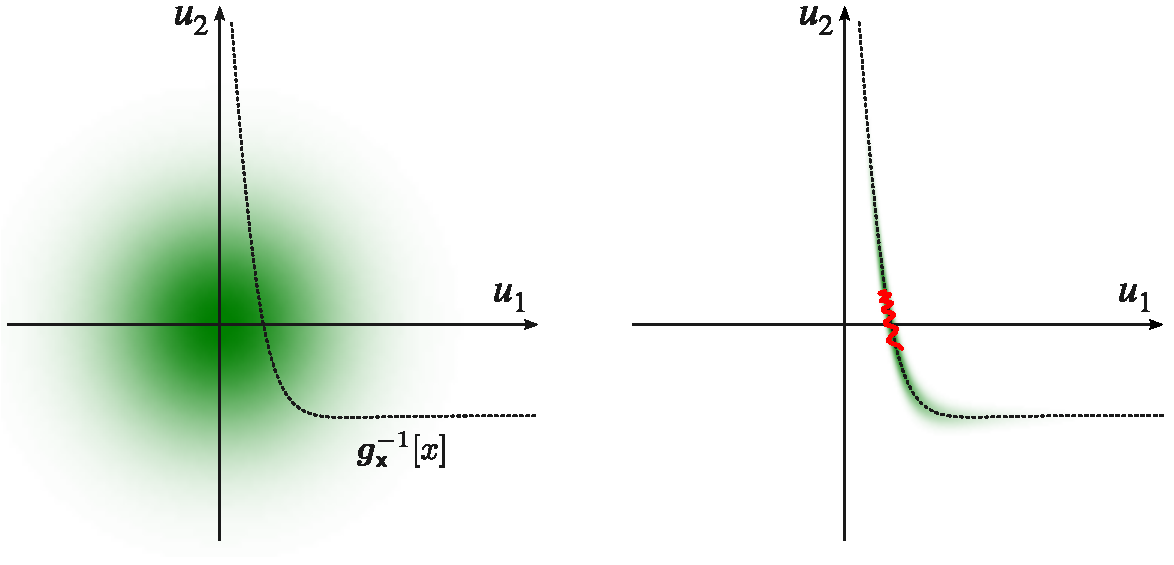
\includegraphics[width=0.8\textwidth]{images/gaussian-abc-with-hmc-trajectory-gray}
\caption[Oscillatory Hamiltonian trajectory example.]{Illustration of oscillatory behaviour in \ac{HMC} trajectories when using an \ac{ABC} target density \eqref{eq:abc-density-input-space} in the input space to a generative model. The left axis shows the two-dimensional input space $\set{U}$ of a toy differentiable generative model with a Gaussian input density $\rho$ (green shading). The dashed curve shows the one-dimensional manifold corresponding to the pre-image under the generator function $\genfunc_{\rvar{x}}$ of an observed output $x$. The right axis shows the same input space with now the green shading showing the density proportional to $k_\epsilon\lpa x; \genfunc_{\rvar{x}}(\vct{u})\rpa \,\rho(\vct{u})$ with a Gaussian $k_\epsilon$. The red curve shows a simulated \ac{HMC} trajectory using this density as the target distribution: the large magnitude density gradients normal to the manifold cause high-frequency oscillations and slows movement along the manifold (which corresponds to variation in the latent variable $\rvar{z}$).}
\label{fig:gaussian-abc-hmc-trajectory-example}
\end{figure}

The requirement for $\preimage{\genfunc_{\rvct{x}}}{\vct{x}}$ to be connected will generally be much more difficult to verify. If the pre-image consists of multiple disconnected components then the dynamic will generally remain confined to just one of them. Although problematic, this issue is similar to that faced by most \ac{MCMC} methods in target distributions which potentially have multiple separated modes. Defining an augmented generator $\genfunc_{\rvct{y}}(\rvct{u},\rvct{n}) = \genfunc_{\rvct{x}}(\rvct{u}) + \epsilon \rvct{n}$ with $\rvct{n}$ a vector of $N_{\rvct{x}}$ independent zero-mean unit-variance Gaussian random variables and $\epsilon$ a small constant and then performing constrained \ac{HMC} on the augmented pair $(\rvct{u},\rvct{n})$ will guarantee that the manifold $\preimage{\genfunc_{\rvct{y}}}{\vct{x}}$ is connected and $\jacobian{\genfunc_{\rvct{y}}}$ is full row-rank everywhere. Of course this is equivalent to the \ac{ABC} approach with a $\epsilon$ tolerance Gaussian kernel, and using our earlier observation we could alternatively perform standard \ac{HMC} in the input space using \eqref{eq:abc-density-input-space} as the target density. 

If $\epsilon$ is small however the high gradients in the target density normal to the tangent space of the manifold $\preimage{\genfunc_{\rvct{x}}}{\vct{x}}$ will tend to lead to a small integrator step size needing to be used to maintain reasonable accept rates and the simulated trajectories tend to exhibit high frequency oscillations as illustrated in Figure \ref{fig:gaussian-abc-hmc-trajectory-example}. We have found in some cases that applying constrained \ac{HMC} with the Gaussian augmented generator $\genfunc_{\rvct{y}}$ can therefore still be more efficient than running standard \ac{HMC} in the \ac{ABC} target density, despite the much higher per-step costs, as constrained \ac{HMC} updates are able to make much larger steps, particularly when using small $\epsilon$. The constrained \ac{HMC} dynamic exploits more information about the geometry of the target distribution by using the Jacobian $\jacobian{\genfunc{\rvct{x}}}$ which describes the tangent space of the manifold. A related approach would be to use a Riemannian-manifold \ac{HMC} \citep{girolami2011riemann} method with a position-dependent metric $\mtx{M}(\vct{u}) = \jacob{\genfunc_{\rvct{x}}}{\vct{u}}\jacob{\genfunc_{\rvct{x}}}{\vct{u}}\phantom{}\tr + \epsilon^2\mathbf{I}$ when using a Gaussian \ac{ABC} kernel in the input space (equation \eqref{eq:abc-density-input-space}); this should dynamically adjust the momentum scaling so as to reduce the inefficient oscillatory behaviour seen in the standard (fixed metric) \ac{HMC} trajectories \cite{betancourt2013general}.

\section{Method}\label{sec:method}

Our constrained \ac{HMC} implementation is shown in Algorithm \ref{alg:constrained_hmc}. We use a generalisation of the RATTLE scheme to simulate the dynamic. The inner updates of the state to solve for the geodesic motion on the constraint manifold are split into multiple smaller steps, which is a special case of the scheme described in \citep{leimkuhler2016efficient}. This allows more flexibility in choosing an appropriately small step-size to ensure convergence of the iterative solution of the equations projecting on to the constraint manifold while still allowing a more efficient larger step size for updates to the momentum due to the negative log density gradient. We have assumed $\mtx{M} = \mtx{I}$ here; other mass matrix choices can be equivalently implemented by adding an initial linear transformation stage in the generator.

\begin{algorithm}[!t]
\caption{Constrained Hamiltonian Monte Carlo}
\label{alg:constrained_hmc}
{
\small
\begin{algorithmic}
\small
    \Require\\
    $\genfunc_{\rvct{x}}$ : observed variable generator function; \\
    $\phi$ : potential energy function $\phi(\vct{u}) = -\log\rho(\vct{u}) + \frac{1}{2}\log|\jacob{\genfunc_{\vct{x}}}{\vct{u}}\jacob{\genfunc_{\vct{x}}}{\vct{u}}|$;\\
    $\vct{x}$ : observed data values being conditioned on; \\
    $\vct{u}$ : current chain state (model inputs) with $\Vert\genfunc_{\rvct{x}}(\vct{u}) - \vct{x}\Vert_\infty < \epsilon$;\\% and $\jacob{\genfunc_{\rvct{x}}}{\vct{u}}\vct{p} = \vct{0}$; \\
    %$\varphi$ : cached value of potential energy $\phi$ evaluated at $\vct{u}$ in previous transition;\\
    $(\varphi, \mtx{J}, \mtx{L})$ : cached values of $\phi$, $\jacobian{\genfunc_{\rvct{x}}}$ and $\chol\lpa\jacobian{\genfunc_{\rvct{x}}}\jacobian{\genfunc_{\rvct{x}}}\phantom{}\tr\rpa$ evaluated at $\vct{u}$; \\
    $\epsilon$ : convergence tolerance for Newton iteration;\\
    $M$ : number of Newton iterations to try before rejecting for non-convergence; \\
    $\delta t$ : integrator time step; \\
    $N_s$ : number of time steps to simulate; \\
    $N_g$ : number of geodesic steps per time step.
    \Ensure\\
    $\vct{u}_{\mathrm{n}}$ : new chain state with $\Vert\genfunc_{\rvct{x}}(\vct{u}_{\textrm{n}}) - \vct{x}\Vert_\infty < \epsilon$; \\% and $\jacob{\genfunc_{\rvct{x}}}{\vct{u}'}\vct{p}' = \vct{0}$; \\
    $(\varphi_{\textrm{n}},\mtx{J}_{\mathrm{n}}, \mtx{L}_{\mathrm{n}})$ : values of $\phi$, $\jacobian{\genfunc_{\rvct{x}}}$ and $\chol\lpa\jacobian{\genfunc_{\rvct{x}}}\jacobian{\genfunc_{\rvct{x}}}\phantom{}\tr\rpa$ evaluated at new $\vct{u}_{\textrm{n}}$.
\end{algorithmic}
\vspace{1mm}
\hrule
\begin{multicols}{2}
\small
\begin{algorithmic}
    \State $\vct{n} \sim \nrm{\vct{0},\mathbf{I}}$
    \State $\vct{p} \gets \Call{ProjectMom}{\vct{n},\mtx{J},\mtx{L}}$
    \State $\vct{u}_{\mathrm{p}},\vct{p}_{\mathrm{p}},\mtx{J}_{\mathrm{p}},\mtx{L}_{\mathrm{p}} \gets \Call{SimDyn}{\vct{u},\vct{p},\mtx{J},\mtx{L}}$
    \State $\varphi_{\mathrm{p}} \gets \phi(\vct{u})$
    %$\varphi_{\mathrm{p}} \gets \sum_{i=1}^{N_{\rvct{x}}}\lpa \log [\mtx{L}_{\mathrm{p}}]_{i,i} \rpa - \log\rho(\vct{u}_{\mathrm{p}})$
    \State $r \sim \mathcal{U}(0,1)$
    \State $p_a \gets \exp\lpa \varphi + \frac{1}{2}\vct{p}\tr\vct{p} - \varphi_{\mathrm{p}} - \frac{1}{2}\vct{p}_{\mathrm{p}}\tr\vct{p}_{\mathrm{p}} \rpa$
    \If{$r < p_a$}
        \State $\vct{u}_{\mathrm{n}},\varphi_{\textrm{n}},\mtx{J}_{\mathrm{n}},\mtx{L}_{\mathrm{n}} 
        \gets \vct{u}_{\mathrm{p}},\varphi_{\mathrm{p}},\mtx{J}_{\mathrm{p}},\mtx{L}_{\mathrm{p}}$
    \Else
        \State $\vct{u}_{\mathrm{n}},\varphi_{\mathrm{n}},\mtx{J}_{\mathrm{n}},\mtx{L}_{\mathrm{n}} 
        \gets \vct{u},\varphi,\mtx{J},\mtx{L}$
    \EndIf
    \State % empty line 
    \Function{SimDyn}{$\vct{u}$, $\vct{p}$, $\mtx{J}$, $\mtx{L}$}
        \State $\tilde{\vct{p}} \gets \vct{p} - \frac{\delta t}{2} \nabla\phi({\vct{u}})$
        \vspace{0.5mm}
        \State $\vct{p} \gets \Call{ProjectMom}{\tilde{\vct{p}},\mtx{J},\mtx{L}}$
        \State $\vct{u},\vct{p},\mtx{J},\mtx{L} \gets \Call{SimGeo}{\vct{u},\vct{p},\mtx{J},\mtx{L}}$
        \For{$s \in \fset{2 \dots N_s}$}
            \State $\tilde{\vct{p}} \gets \vct{p} - \delta t \nabla\phi({\vct{u}})$
            \vspace{0.5mm}
            \State $\vct{p} \gets \Call{ProjectMom}{\tilde{\vct{p}},\mtx{J},\mtx{L}}$
            \State $\vct{u},\vct{p},\mtx{J},\mtx{L} \gets \Call{SimGeo}{\vct{u},\vct{p},\mtx{J},\mtx{L}}$
        \EndFor
        \State $\tilde{\vct{p}}\gets \vct{p} - \frac{\delta t}{2} \nabla\phi({\vct{u}})$
        \vspace{0.5mm}
        \State $\vct{p} \gets \Call{ProjectMom}{\tilde{\vct{p}},\mtx{J},\mtx{L}}$
        \State \Return $\vct{u},\vct{p},\mtx{J},\mtx{L}$
    \EndFunction
    \State % empty line
    \Function{ProjectMom}{$\vct{p}$, $\mtx{J}$, $\mtx{L}$}
        \State \Return $\vct{p} - \mtx{J}\tr\mtx{L}^{-\textsf{T}}\mtx{L}^{-1}\mtx{J}\vct{p}$
    \EndFunction
    \columnbreak
    \Function{ProjectPos}{$\vct{u}$, $\mtx{J}$, $\mtx{L}$}
         \State $\vct{\delta} \gets \genfunc_{\rvct{x}}(\vct{u}) - \vct{x}$
         \State $i \gets 0$
         \While{$\Vert\vct{\delta}\Vert_{\infty} > \epsilon \,\land\, i < M$}
         \label{ln:convergence-check}
             \State $\vct{u} \gets \vct{u} - \mtx{J}\tr \mtx{L}^{-\textsf{T}} \mtx{L}^{-1} \vct{\delta}$
             \State $\vct{\delta} \gets \genfunc_{\rvct{x}}(\vct{u}) - \vct{x}$
             \State $i \gets i + 1$
         \EndWhile
         \If{$i = M$} 
           \State \textbf{raise}  \textsc{RejectMove} \label{ln:non-convergence} 
         \EndIf
         \State \Return $\vct{u}$
    \EndFunction
    \State % empty line
    \vspace{-2mm}
    \Function{SimGeo}{$\vct{u}$, $\vct{p}$, $\mtx{J}$, $\mtx{L}$}
        \For{$i \in \fset{1 \dots N_g}$}
            \State $\tilde{\vct{u}} \gets \vct{u} + \frac{\delta t}{N_g} \,\vct{p}$
            \State $\vct{u}' \gets \Call{ProjectPos}{\tilde{\vct{u}}, \mtx{J}, \mtx{L}}$
            \State $\mtx{J} \gets \jacob{\genfunc_{\rvct{x}}}{\vct{u}'}$
            \State $\mtx{L} \gets \chol \lpa \mtx{J}\mtx{J}\tr \rpa$ \label{ln:chmc-cholesky}
            \State $\tilde{\vct{p}} \gets \frac{N_g}{\delta t}\lpa \vct{u}' - \vct{u} \rpa$
            \State $\vct{p} \gets \Call{ProjectMom}{\tilde{\vct{p}},\mtx{J},\mtx{L}}$
            \State $\vct{u}_r \gets \vct{u}' - \frac{\delta t}{N_g} \vct{p}$
            \State $\vct{u}_r \gets \Call{ProjectPos}{\vct{u}_r, \mtx{J}, \mtx{L}}$
            \If{$\left\Vert \vct{u} - \vct{u}_r \right\Vert_{\infty} > \sqrt{\epsilon}$}
              \State \textbf{raise} \textsc{RejectMove}\label{ln:reverse-check}
            \EndIf
            \State $\vct{u} \gets \vct{u}'$
        \EndFor        
        \State \Return $\vct{u},\vct{p},\mtx{J},\mtx{L}$
    \EndFunction
\end{algorithmic}
\end{multicols}
}
\end{algorithm}

Each inner geodesic time-step involves stepping along the current momentum  $\tilde{\vct{u}} \gets \vct{u} + (\nicefrac{\delta t}{N_g}) \vct{p}$ and then projecting $\tilde{\vct{u}}$ back on to $\preimage{\genfunc_{\rvct{x}}}{\vct{x}}$ by solving for $\vct{\lambda}$ which satisfy $\genfunc_{\rvct{x}}(\tilde{\vct{u}} - \mtx{J}\tr\vct{\lambda}) = \vct{x}$ where $\mtx{J} = \jacob{\genfunc_{\rvct{x}}}{\vct{u}}$. This is performed in the function \textsc{ProjectPos} in Algorithm \ref{alg:constrained_hmc}. Here we use a quasi-Newton method for solving the system of equations. The true Newton update would be
\begin{equation}\label{eq:newton-iteration}
    \vct{u}'\gets \vct{u}' - 
    \mtx{J}\tr
    \lpa 
        \jacob{\genfunc_{\rvct{x}}}{\vct{u}'}\mtx{J}\tr
    \rpa^{-1}
    \lpa \genfunc_{\rvct{x}}(\vct{u}') - \vct{x} \rpa.
\end{equation}
This requires recalculating the Jacobian and solving a dense linear system within the optimisation loop. Instead we use a symmetric quasi-Newton update, 
\begin{equation}\label{eq:quasi-newton-iteration}
    \vct{u}'\gets \vct{u}' - 
    \mtx{J}\tr
    \lpa 
        \mtx{J}\mtx{J}\tr
    \rpa^{-1}
    \lpa \genfunc_{\rvct{x}}(\vct{u}') - \vct{x} \rpa.
\end{equation}
as proposed in \citep{barth1995algorithms}. The Jacobian product $\mtx{J}\mtx{J}\tr$ evaluated at the previous state is used to condition the moves. This matrix is positive-definite and a Cholesky decomposition can be calculated outside the optimisation loop allowing cheaper quadratic cost solves within the loop. 

Convergence of the quasi-Newton iteration is signalled when $\Vert \genfunc_{\rvct{x}}(\vct{u}) - \vct{x}\Vert_\infty < \epsilon$, i.e. the elementwise maximum absolute difference between the model observed output and the observed data is below a tolerance $\epsilon$. The tolerance is analogous to the $\epsilon$ parameter in \ac{ABC} methods, however here we can set this value close to machine precision (with $\epsilon = 10^{-8}$ in the experiments) and so the error introduced is comparable to that otherwise incurred for using non-exact arithmetic.

In some cases the quasi-Newton iteration will fail to converge. We use a fixed upper limit on the number of iterations and reject the move (line \ref{ln:non-convergence} in Algorithm \ref{alg:constrained_hmc}) if convergence is not achieved within this limit. To ensure reversibility, once we have solved for a forward geodesic step on the manifold in \textsc{SimGeo}, we then check if the corresponding reverse step (with the momentum negated) returns to the original position. This involves running a second Newton iteration, though as it reuses the same Jacobian $\mtx{J}$ and Cholesky decomposition $\mtx{L}$, the evaluation of which tend to be the dominant costs in the algorithm, in the experiments we found the overhead introduced tended to be quite small (around a 20\% increase in run-time compared to only performing the forward step). A similar scheme for ensuring reversibility is proposed in \citep{zappa2017monte}. The square root of the tolerance $\epsilon$ used for the initial Newton convergence check \emph{in the output space of generator} (line \ref{ln:convergence-check} in Algorithm \ref{alg:constrained_hmc}) is used for the reverse-step check on \emph{the inputs} (line \ref{ln:reverse-check} in Algorithm \ref{alg:constrained_hmc}) based on standard recommendations for checking convergence in optimisation routines \citep{christensen2008devil}. In the implementation we used in the experiments, we fall back to a \textsc{minpack} \citep{more1980user} implementation of the robust Powell's Hybrid method \citep{powell1970hybrid} if the quasi-Newton iteration diverges or fails to converge, with a rejection then only occurring if both iterative solvers fail. In practice we found if the step size $\delta t$ and number of geodesic steps $N_g$ is chosen appropriately then rejections due to non-convergence / non-reversible steps occur very rarely.

For larger systems, the Cholesky decomposition of the constraint Jacobian matrix product $\jacobian{\genfunc_{\rvct{x}}}\jacobian{\genfunc_{\rvct{x}}}\phantom{}\tr$ (line \ref{ln:chmc-cholesky}) will become a dominant cost, generally scaling cubically with $N_{\rvct{x}}$. In many models however conditional independency structure will mean that not all observed variables $\rvct{x}$ are dependent on all of the input variables $\rvct{u}$ and so the Jacobian $\jacobian{\genfunc_{\rvct{x}}}$ has sparsity structure which can be exploited to reduce this worst-case cost. 

\begin{figure}[!t]
\centering
\begin{subfigure}[t]{.35\linewidth}
\centering
\begin{tikzpicture}
  \node[latent] (z) {$\rvct{z}$} ; %
  \op[above=of z] {uz-z} {right: $\vctfunc{g}_{\rvct{z}}$} {} {z} ; %
  \node[latent, left=0.3 of uz-z] (uz) {$\rvct{u}_1$} ; %
  \factor[left=of uz] {pr-uz} {below: $\rho_{\scriptscriptstyle 1}$} {} {uz} ; %
  \draw (uz) -- (uz-z) ; %
  \node[obs, below=1.2 of z] (xi) {$\rvct{x}_i$} ; %
  \op[above=of xi] {uxi_z-xi} {right:$\vctfunc{g}_{ \rvct{x}_i|\rvct{z}}$} {z} {xi} ; %
  \node[latent, left=0.3 of uxi_z-xi] (uxi)  {$\rvct{u}_{2,i}$} ; %
  \factor[left=of uxi] {pr-uxi} {below: $\rho_{\scriptscriptstyle 2,i}$} {} {uxi} ; %
  \draw (uxi) -- (uxi_z-xi) ; %
  \node[below=0.0 of xi, yshift=0.5mm] (dummy) {} ; %
  \plate {obs} 
    {(xi)(uxi)(uxi_z-xi)(uxi_z-xi-caption)(pr-uxi)(pr-uxi-caption)(dummy)} 
    {\footnotesize $i \in \fset{1 \,...\, N}$} ; %
\end{tikzpicture}
\caption{Independent $\rvct{x}_i$}\label{sfig:directed-model-independent}
\end{subfigure}%
%\begin{subfigure}[t]{.25\linewidth}
%\centering
%\begin{tikzpicture}
%  \node (dummy) {};%
%  \node[latent, below right=1 and 0.2 of dummy] (z) {$\rvct{z}$} ; %
%  \factor[above=of z] {pr-z} {right: \small $\mathsf{p}_{\rvct{z}}$} {} {z} ; %
%  \node[obs, below=1.2 of z] (xi) {$\rvct{x}_i$} ; %
%  \factor[above=of xi] {z-xi} {right:\small $\mathsf{p}_{\rvct{x}_i|\rvct{z}}$} {z} {xi} ; %
%  \node[above=0.1 of z-xi] (dummy2) {} ; %
%  \plate {obs} 
%    {(xi)(z-xi)(z-xi-caption)(dummy2)} 
%    {\tiny $i \in \fset{1 \,...\, N}$} ; %
%\end{tikzpicture}
%\caption{}\label{sfig:directed-model-independent-marginalised}
%\end{subfigure}%
\begin{subfigure}[t]{.62\linewidth}
\centering
\begin{tikzpicture}
  \node[latent] (z) {$\rvct{z}$} ; %
  \op[above=of z] {uz-z} {right: $\vctfunc{g}_{\rvct{z}}$} {} {z} ; %
  \node[latent, left=0.3 of uz-z] (uz) {$\rvct{u}_1$} ; %
  \factor[left=of uz] {pr-uz} {below: $\rho_{\scriptscriptstyle 1}$} {} {uz} ; %
  \draw (uz) -- (uz-z) ; %
  \node[latent, below=1.2 of z] (uone) {$\rvct{u}_{2,1}$} ; %
  \factor[below=of uone] {pr-uone} {right:$\rho_{2,1}$} {} {uone} ; %
  \op[above=of uone] {xzero_uone_z-xone} {below right:$\vctfunc{f}_1$} {} {} ; %
  \node[obs, left=0.3 of xzero_uone_z-xone] (xzero)  {$\rvct{x}_{0}$} ; %
  \op[left=of xzero] {uzero-xzero} {below right: $\vctfunc{f}_0$} {} {xzero} ; %
  \node[latent] (uzero) at (uone-|uzero-xzero) {$\rvct{u}_{2,0}$} ; %
  \factor[below=of uzero] {pr-uzero} {right:$\rho_{2,0}$} {} {uzero} ; %
  \draw (uzero) -- (uzero-xzero) ; %
  \draw (z) -- (uzero-xzero) ; %
  \node[obs, right=0.3 of xzero_uone_z-xone] (xone)  {$\rvct{x}_{1}$} ; %
  \factoredge {xzero,uone,z} {xzero_uone_z-xone} {xone} ; %
  \op[right=0.3 of xone] {xone_utwo_z-xtwo} {below right:$\vctfunc{f}_2$} {} {} ; %  
  \node[latent] (utwo) at (uone-|xone_utwo_z-xtwo) {$\rvct{u}_{2,2}$} ; %
  \factor[below=of utwo] {pr-utwo} {right:$\rho_{2,2}$} {} {utwo} ; %
  \node[obs, right=0.3 of xone_utwo_z-xtwo] (xtwo) {$\rvct{x}_2$} ; %
  \factoredge {z,xone,utwo} {xone_utwo_z-xtwo} {xtwo} ; %
  \node[right=0.1 of xtwo] (dummy) {} ; %
  \draw[densely dotted] (xtwo) -- (dummy) ; %
  \op[right=0.5 of xtwo] {ufinal-xfinal} {below right:$\vctfunc{f}_T$} {} {} ; %  
  \node[latent] (ufinal) at (uone-|ufinal-xfinal) {$\rvct{u}_{2,T}$} ; %
  \factor[below=of ufinal] {pr-ufinal} {right:$\rho_{2,T}$} {} {ufinal} ; %
  \node[obs, right=0.3 of ufinal-xfinal] (xfinal) {$\rvct{x}_T$} ; %
  \factoredge {ufinal} {ufinal-xfinal} {xfinal} ; %
  \node[left=0.1 of ufinal-xfinal] (dummy2) {} ; %
  \draw[densely dotted] (dummy2) -- (ufinal-xfinal) ; %
  \node[above left=0.1 and 0.2 of ufinal-xfinal] (dummy3) {} ; %
  \draw[densely dotted] (dummy3) -- (ufinal-xfinal) ; %
\end{tikzpicture}
\caption{Markovian $\rvct{x}_i$}\label{sfig:directed-model-markov}
\end{subfigure}%
\caption[Structured directed generative models.]{Factor graphs of examples of structured directed generative models.}
\label{fig:directed-model-structure-examples}
\end{figure}

In particular two common cases are directed generative models in which the observed variables $\rvct{x}$ can be split into groups $\fset{\rvct{x}_i}_{i=1}^G$ such that all of the $\rvct{x}_i$ are either conditionally independent given the latent variables $\rvct{z} = \genfunc_{\rvct{z}}(\rvct{u}_1)$ (for example independent and identically distributed observations), or each $\rvct{x}_i$ is conditionally independent of all $\lbrace \rvct{x}_j \rbrace_{j<i-1}$ given $\rvct{x}_{i-1}$ and $\rvct{z}$ (most commonly Markov chains for example from a \ac{SDE} model though observations with more general tree structured dependencies can also be ordered into this form). Figure \ref{fig:directed-model-structure-examples} shows factor graphs for directed generative models with these two structures, with the conditional independencies corresponding to each $\rvct{x}_i$ being generated as a function of only a subset $\rvct{u}_{2,i}$ of the random input variables $\rvct{u}_2$. Equivalently these structures correspond to generator functions $\genfunc_{\rvct{x}}$ which can be expressed in one of the two forms
\begin{align}\label{eq:elem_autoreg_model_struct}
    \rvct{x}_i &= \genfunc_{\rvct{x}_i|\rvct{z}}(\rvct{z}, \rvct{u}_{2,i})
    & \text{(independent)}\\
    \rvct{x}_{i} 
    &=
    \vctfunc{f}_i\lpa\rvct{z}, \rvct{x}_{i-1}, \rvct{u}_{2,i}\rpa = 
    \genfunc_{\rvct{x}_i|\rvct{z}}\lpa\rvct{z}, \lbrace\rvct{u}_{2,j}\rbrace^i_{j=1}\rpa & \text{(Markov).}
\end{align}
For models with these structures the generator Jacobian
\begin{equation}
  \jacobian{\genfunc_{\rvct{x}}} =
  \lsb
   \pd{\genfunc_{\rvct{x}}}{\vct{u}_1} \,\middle|\,
   \pd{\genfunc_{\rvct{x}}}{\vct{u}_2}
  \rsb
\end{equation}
has a component $\pd{\genfunc_{\rvct{x}}}{\vct{u}_2}$ which is either block-diagonal (independent) or block-triangular (Markovian). Considering first the simplest case where each $(\rvct{x}_i,\rvct{u}_{2,i})$ pair are single dimensional, the Cholesky decomposition of $\jacobian{\genfunc_{\rvct{x}}}\jacobian{\genfunc_{\rvct{x}}}\phantom{}\tr = \pd{\genfunc_{\rvct{x}}}{\vct{u}_1}\pd{\genfunc_{\rvct{x}}}{\vct{u}_1}\tr + \pd{\genfunc_{\rvct{x}}}{\vct{u}_2} \pd{\genfunc_{\rvct{x}}}{\vct{u}_2}\tr$ can then be computed by low-rank Cholesky updates of the triangular / diagonal matrix $\pd{\genfunc_{\rvct{x}}}{\vct{u}_2}$ with each of the columns of $\pd{\genfunc_{\rvct{x}}}{\vct{u}_1}$. As $\dim(\vct{u}_1) = L$ is often significantly less than the number of observations being conditioned on $N_{\rvct{x}}$, the resulting $\mathcal{O}(LN_{\rvct{x}}^2)$ cost of the low-rank Cholesky updates is a significant improvement over the original $\mathcal{O}(N_{\rvct{x}}^3)$. For cases in which each $(\rvct{x}_i,\rvct{u}_{2,i})$ pair are both vectors of dimension $D$ (i.e. $N_{\rvct{x}} = GD$) and so $\pd{\genfunc_{\rvct{x}}}{\vct{u}_2}$ is block diagonal / triangular, then the Cholesky factorisation of  $\pd{\genfunc_{\rvct{x}}}{\vct{u}_2} \pd{\genfunc_{\rvct{x}}}{\vct{u}_2}\phantom{}\tr$ can be computed at a cost $\mathcal{O}(G D^3)$ for block diagonal, and $\mathcal{O}(G^2 D^3)$ for block triangular $\pd{\genfunc_{\rvct{x}}}{\vct{u}_2}$, with then again $\mathcal{O}(LN_{\rvct{x}}^2)$ cost low-rank updates of this Cholesky factor by the columns of $\pd{\genfunc_{\rvct{x}}}{\vct{u}_1}$ performed. When $\rvct{x}_i$ and $\rvct{u}_{2,i}$ are vectors of differing dimensions, with generally in this case $\dim(\rvct{u}_{2,i}) > \dim(\rvct{x}_{i})$ due to the requirement the total number of random inputs $M$ is at least $N_{\rvct{x}}$, then though we could choose a subset of each $\rvct{u}_{2,i}$ of equal dimension to $\rvct{x}_i$ so as to identify a block-triangular component, generally any gain from exploiting this structure will be minimal and in practice it seems likely to be more efficient to compute the Cholesky of $\jacobian{\genfunc_{\rvct{x}}}\jacobian{\genfunc_{\rvct{x}}}\phantom{}\tr$ directly.

%Many learnt differentiable generative models have the element-wise noise structure including the Gaussian \ac{VAE}. The autoregressive noise structure commonly occurs in stochastic dynamical simulations where the outputs are a time sequence of states, with noise being added each time-step, for example the Lotka-Volterra model considered in the experiments in Section \ref{sec:experiments}.

The Metropolis accept step and momentum updates in the \textsc{SimDyn} routine require evaluating the logarithm of the target density \eqref{eq:tgt-density-on-manifold} and its gradient respectively. Although this can by achieved by directly using the expression given in \eqref{eq:tgt-density-on-manifold} (and applying reverse-mode \ac{AD} to get the gradient), both the log-density and gradient can be more efficiently calculated by reusing the Cholesky decomposition of the constraint Jacobian Gram matrix computed in line \ref{ln:chmc-cholesky}. Details are given in Appendix \ref{sec:tgt-density-grad}.

A final implementation detail is the requirement to find an initial $\vct{u}$ satisfying $\genfunc_{\rvct{x}}(\vct{u}) = \vct{x}$. In directed generative models with one of the structures just described, one method we found worked well in the experiments was to sample a $\vct{u}_1$, $\vct{u}_2$ pair from $P$ and then keeping the $\vct{u}_1$ values fixed, solve $\genfunc_{\rvct{x}}\lpa\genfunc_{\rvct{z}}(\vct{u}_1),\,\vct{u}_2\rpa= \vct{x}$ for $\vct{u}_2$ using for example Newton's method or by directly minimising the Euclidean norm $\Vert\genfunc_{\rvct{x}}\lpa\genfunc_{\rvct{z}}(\vct{u}_1),\,\vct{u}_2\rpa - \vct{x}\Vert_2^2$ with respect to $\vct{u}_2$ by gradient descent. In more general cases one possible strategy is to randomly sample affine subspaces by generating a $M \times N_{\rvct{x}}$ matrix $\mtx{P}$ and $M$ dimensional vector $\vct{b}$ and then attempting to find any intersections with the manifold by iteratively solving $\genfunc_{\vct{x}}\lpa\mtx{P}\vct{v} + \vct{b}\rpa$ for $\vct{v}$ (and sampling a new subspace if no roots are found).


%For general generators, we can choose a subset of the inputs (or linear projections of the inputs) of dimensionality $N_{\rvct{x}}$ and plug the resulting system of equations into a black-box solver.

\section{Related work}\label{sec:related-work}

Closely related is the \emph{Constrained \ac{HMC}} method of \citep{brubaker2012family}, which demonstrates the validity of the constrained \ac{HMC} framework theoretically and experimentally. The proposed method in \citep{brubaker2012family} uses a RATTLE-based integrator rather than the geodesic scheme used here. The focus in \citep{brubaker2012family} is also on performing inference in distributions inherently defined on a fixed non-Euclidean manifold such as the unit sphere or space of orthogonal matrices, rather than performing inference in differentiable generative models. %Our work builds on \citep{brubaker2012family} by highlighting that conditioning on the output of a generator imposes a constraint on its inputs and so defines a density in input space restricted to some manifold. Unlike the cases considered in \citep{brubaker2012family} our constraints are therefore data-driven and the target density on the manifold implicitly defined by a generator function and base density.

\emph{Geodesic Monte Carlo} \citep{byrne2013geodesic} also considers applying a \ac{HMC} scheme to sample from non-linear manifolds embedded in a Euclidean space. Similarly to \citep{brubaker2012family} however the motivation is performing inference with respect to distributions explicitly defined on a manifold such as directional statistics. The method presented in \citep{byrne2013geodesic} uses an exact solution for the geodesic flow on the manifold. Our use of constrained Hamiltonian dynamics, and in particular the geodesic integration scheme of \citep{leimkuhler2016efficient}, can be considered an extension for cases when an exact geodesic solution is not available. Instead the geodesic flow is approximately simulated while still maintaining the required volume-preservation and reversibility properties for validity of the overall \ac{HMC} scheme.

An alternative Metropolis method for sampling from densities defined on manifolds embedded in a Euclidean space is proposed in \citep{zappa2017monte}. Compared to constrained \ac{HMC} this alleviates the requirements to calculate the gradient of (the logarithm of) the target density on the manifold, though still requiring evaluation of the constraint function Jacobian. As discussed earlier in Section \ref{sec:differentiable-generative-models} (and in Appendix \ref{sec:tgt-density-grad}), using reverse-mode \ac{AD} the gradient of the target density can be computer at a constant factor overhead of evaluating the target density itself. In general we would expect exploiting the gradient of the target density on the manifold within a simulated Hamiltonian dynamic to lead to more coherent exploration of the target distribution, instead of the more random-walk behaviour of a non-gradient based Metropolis update, and so for the gradient evaluation overhead to be worthwhile.

There is extensive theoretical discussion of the issues involved in sampling from distributions defined on manifolds in \citep{diaconis2013sampling}, including a derivation of the conditional density on a manifold using the co-area formula which directly motivated our earlier derivation of the target density for our constrained \ac{HMC} method. The experiments in \citep{diaconis2013sampling} are mainly concentrated on expository examples using simple parameterised manifolds such as a torus embedded in $\reals^3$ and conditional testing in exponential family distributions. 

%In our setting the gradient of the logarithm of the target density on the manifold \eqref{eq:tgt-density-on-manifold} consists of the sum of $\grad\log\rho$ and $-\frac{1}{2}\nabla\log\left|\jacobian{\genfunc_{\rvct{x}}}\jacobian{\genfunc_{\rvct{x}}}\phantom{}\tr\right|$. The former will typically be cheap compute and as shown in the Appendix the latter can be efficiently computed 

\emph{Hamiltonian ABC} \cite{meeds2015hamiltonian}, also proposes applying \ac{HMC} to perform inference in simulator models as considered here. An {ABC} set-up is used with a Gaussian synthetic-likelihood formed by estimating moments from simulated data. Rather than using automatic differentiation to exactly calculate gradients of the generator function, \emph{Hamiltonian ABC} uses a stochastic gradient estimator. This is based on previous work considering methods for using a stochastic gradients within \ac{HMC} \citep{welling2011bayesian,chen2014stochastic}. It has been suggested however that the use of stochastic gradients can destroy the favourable properties of Hamiltonian dynamics which enable coherent exploration of high dimensional state spaces \citep{betancourt2015fundamental}. In \emph{Hamiltonian ABC} it is also observed that representing the generative model as a deterministic function by fixing the random inputs to the generator is a useful method for improving exploration of the state space. This is achieved by including the seed of the pseudo-random number generator in the chain state rather than the set of random inputs.

Also related is \emph{Optimisation Monte Carlo} \citep{meeds2015optimization}. The authors propose using an optimiser to find parameters of a simulator model consistent with observed data (to within some tolerance $\epsilon$) given fixed random inputs sampled independently. The optimisation is not volume-preserving and so the Jacobian of the map is approximated with finite differences to weight the samples. Our method also uses an optimiser to find inputs consistent with the observations, however by using a volume-preserving dynamic we avoid having to re-weight samples which can scale poorly with dimensionality. 

Our method also differs in treating all inputs to a generator equivalently; while the \emph{Optimisation Monte Carlo} authors similarly identify the simulator models as deterministic functions they distinguish between parameters and random inputs, optimising the first and independently sampling the latter. This can lead to random inputs being sampled for which no parameters can be found consistent with the observations (even with a within $\epsilon$ constraint). Although optimisation failure is also potentially an issue for our method, we found this occurred rarely in practice if an appropriate step size is chosen. Our method can also be applied in cases were the number of unobserved variables is greater than the number of observed variables unlike \emph{Optimization Monte Carlo}.

\section{Experiments}\label{sec:experiments}

To illustrate the wide applicability of the proposed method we performed inference tasks in three diverse settings: parameter inference in a stochastic Lotka-Volterra predator-prey model simulation, 3D human pose and camera parameter inference given 2D joint position information and finally in-painting of missing regions of digit images using a generative model trained on MNIST. In all three experiments Theano \citep{theano2016theano} was used to specify the generator function and calculate the required derivatives. All experiments were run on an Intel Core i5-2400 quad-core CPU. Python code for the experiments is available at \url{https://git.io/dgm}.

\subsection{Lotka--Volterra parameter inference}

\begin{figure}[!t]
\centering
\begin{subfigure}[b]{0.85\textwidth}
  \centering
  \caption{}
  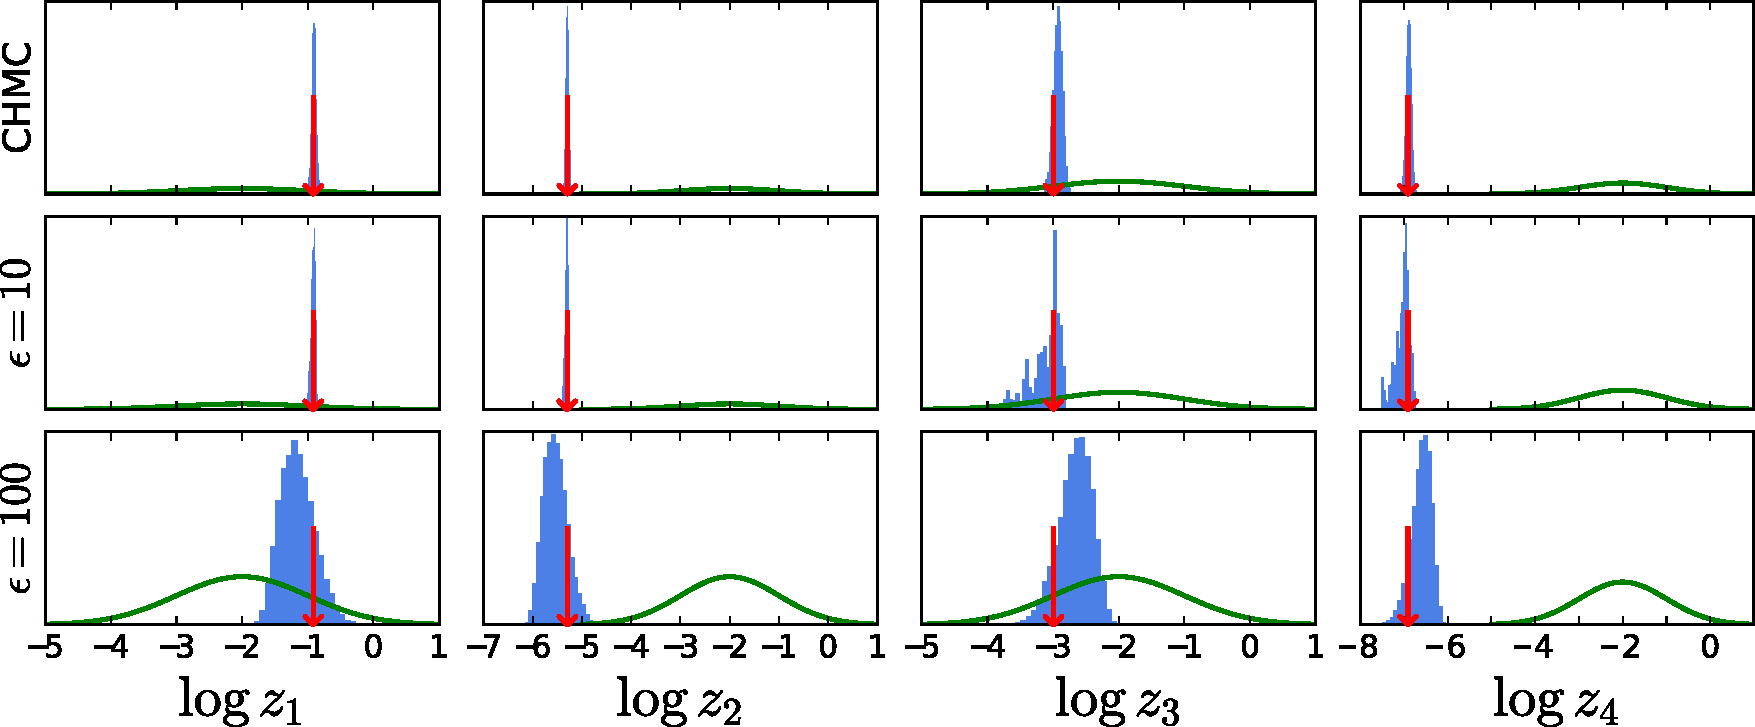
\includegraphics[width=\textwidth]{images/lotka-volterra-marginals-with-prior}
  \label{sfig:lotka-volterra-marginals}
\end{subfigure}\\
\begin{subfigure}[b]{0.33\textwidth}
  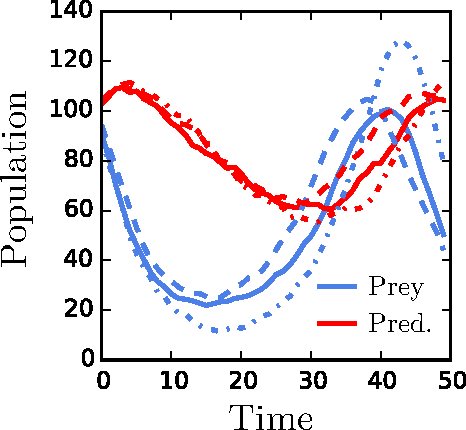
\includegraphics[width=\textwidth]{images/lotka-volterra-sims.pdf}
  \caption{}
  \label{sfig:lotka-volterra-sims}
\end{subfigure}
~~~~
\begin{subfigure}[b]{0.52\textwidth}
  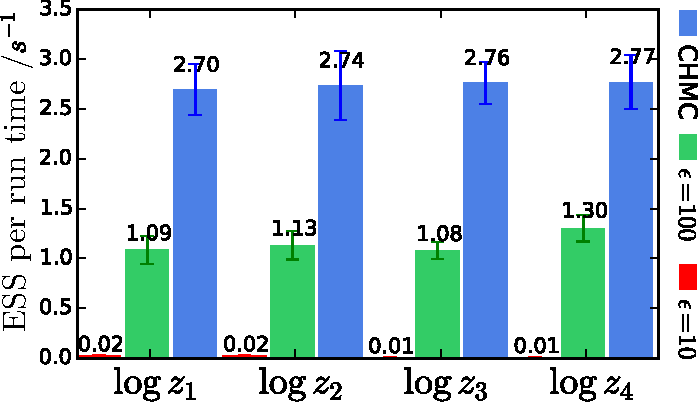
\includegraphics[width=\textwidth]{images/lotka-volterra-ess.pdf}
  \caption{}
  \label{sfig:lotka-volterra-ess}
\end{subfigure}
\caption[Inference in Lotka--Volterra simulator model.]{\textsf{Lotka--Volterra}~~ 
\subref{sfig:lotka-volterra-marginals} Marginal empirical histograms for the (logarithm of the) four parameters (columns) from constrained \ac{HMC} samples (top) and \ac{ABC} samples with $\epsilon=10$ (middle) and $\epsilon=100$ (bottom). Horizontal axes shared across columns. Red arrows indicate true parameter values.  Green curves show the log-normal prior densities for comparison. 
\subref{sfig:lotka-volterra-sims} Observed predator-prey populations (solid) and \ac{ABC} sample trajectories with $\epsilon=10$ (dashed) and $\epsilon=100$ (dot-dashed). 
\subref{sfig:lotka-volterra-ess} Mean \ac{ESS} normalised by compute time for each of four parameters for \ac{ABC} with $\epsilon=10$ (red), $\epsilon=100$ (green) and our method (blue). Error bars show $\pm 3$ standard errors of mean.}
\label{fig:lotka-volterra}
\end{figure}

\begin{algorithm}[t]
\caption{Lotka--Volterra model generator functions}
\label{alg:lotka-volterra-generators}
\begin{algorithmic}
\small
    \Require\\
    $\delta t$ : Euler--Maryuma integrator time step;\\
    $N_s$ : number of integrator steps to perform;\\
    $f, r$ : initial predator and prey populations; \\
    $\sigma$ : white noise process standard deviation; \\
    $\vct{m},\,\vct{s}$ : location and scale parameters of log-normal prior.\\
\end{algorithmic}
\vspace{-1mm}
\hrule
\vspace{1mm}
%\begin{multicols}{2}
\small
\begin{algorithmic}
\Function{$\genfunc_{\rvct{z}}$}{$\rvct{u}_1$}
  \State $\rvct{z} \gets \exp(\vct{s} \,\odot\, \rvct{u}_1 + \vct{m})$
  \State \Return $\rvct{z}$
\EndFunction
\Function{$\genfunc_{\rvct{x}|\rvct{z}}$}{$\rvct{z},\,\rvct{u}_2$}
  \State $\rvar{r}_0 \gets r$  
  \State $\rvar{f}_0 \gets f$
  \For{$s \in \fset{1 \dots N_s}$}
    \State $\rvar{r}_s \gets \rvar{r}_{s-1} + \delta t(\rvar{z}_1 \rvar{r}_{s-1} - \rvar{z}_2 \rvar{r}_{s-1} \rvar{f}_{s-1}) + \sqrt{\delta t} \sigma  \rvar{u}_{2,2s}$
    \State $\rvar{f}_s \gets \rvar{f}_{s-1} + \delta t(\rvar{z}_4 \rvar{r}_{s-1} \rvar{f}_{s-1} - \rvar{z}_3 \rvar{f}_{s-1}) + \sqrt{\delta t} \sigma  \rvar{u}_{2,2s+1}$
  \EndFor
  \State $\rvct{x} \gets \lsb \rvar{r}_1,\, \rvar{f}_1, \,\dots \rvar{r}_{N_s},\,\rvar{f}_{N_s} \rsb$
  \State \Return $\rvct{x}$
\EndFunction
\end{algorithmic}
%\end{multicols}
\end{algorithm}

As a first demonstration we considered a stochastic continuous state variant of the Lotka--Volterra model, a common example problem for \ac{ABC} methods e.g. \citep{meeds2015optimization}. In particular we consider parameter inference given a simulated solution of the following stochastic differential equations
\begin{equation}\label{eq:lotka-volterra}
    \dr r = \lpa z_1 r - z_2 r f \rpa \dr t + \dr n_r,
    \quad
    \dr f = \lpa z_4 r f -z_3 f \rpa \dr t + \dr n_f,
\end{equation}
where $r$ represents the prey population, $f$ the predator population, $\fset{z_i}_{i=1}^4$ the system parameters and $n_r$ and $n_f$ zero-mean white noise processes.

The observed data was generated with an Euler-Maruyama discretisation, time-step $\delta t = 1$, white noise process standard deviation $\sigma = 1$, initial condition $r_0 = f_0 = 100$ and $\rvar{z}_1=0.4$, $\rvar{z}_2 = 0.005$,  $\rvar{z}_3=0.05$, $\rvar{z}_4=0.001$ (chosen to give stable dynamics). The simulation was run for $N_s = 50$ time-steps with the observed outputs defined as the concatenated vector $\rvct{x} = { \lsb \rvar{r}_1 ~ \rvar{f}_1 ~ \dots ~ \rvar{r}_{50} ~ \rvar{f}_{50} \rsb}$. Log-normal priors $\rvar{z}_i \sim \log \nrm{-2, 1}$ were place on the system parameters. Pseudo-code for the corresponding generator functions $\genfunc_{\rvct{z}}$ and $\genfunc_{\rvct{x}|\rvct{z}}$ is given in Algorithm \ref{alg:lotka-volterra-generators}. The generator in this case has the Markovian structure discussed in Section \ref{sec:method} allowing efficient computation of the Cholesky factor of the Jacobian matrix product $\jacobian{\genfunc_{\rvct{x}}}\jacobian{\genfunc_{\rvct{x}}}\tr$.

We compared our method to various \ac{ABC} approaches using a uniform ball kernel with radius $\epsilon$. \ac{ABC} rejection failed catastrophically, with no acceptances in $10^6$ samples even with a large $\epsilon = 1000$. \ac{ABC} \ac{MCMC} with a Gaussian proposal density $q$ also performed very poorly with the dynamic having zero acceptances over multiple runs of $10^5$ updates for $\epsilon=100$ and getting stuck at points in parameter space over many updates for larger $\epsilon=1000$, even with small proposal steps. The same issues were also observed when using a Gaussian kernel. As we are conditioning on all of the observed data without use of summary statistics this poor performance is not unexpected.

We found that however by constructing a chain in the generator inputs space with target distribution \eqref{eq:abc-density-input-space}, we can afford to condition on all of the observed outputs even when using relatively simple non-gradient based \ac{MCMC} methods. In particular based on the pseudo-marginal slice sampling method \citep{murray2010slice} discussed earlier, we tried using alternating elliptical slice sampling updates of the random inputs $\rvct{u}_1$ used to generate the parameters, i.e. $\rvct{z} = \genfunc_{\rvct{z}}(\rvct{u}_1)$, and remaining random inputs $\rvct{u}_2$ used to generate the simulated observations given parameters, i.e. $\rvct{x} = \genfunc_{\rvct{x}|\rvct{z}}(\rvct{z},\rvct{u}_2)$. The slice sampling updates locally adapt the size of steps made to ensure a move can always be made. Using this method we were able to obtain reasonable convergence over long runs for both $\epsilon=100$ and $\epsilon=10$. We therefore used this as our base-line method to compare the gains (in terms of how well the parameters are identified in the posterior) from using an $\epsilon \approx 0$ in the proposed constrained \ac{HMC} method compared to non-zero $\epsilon$ values.

The results are summarised in Figure \ref{fig:lotka-volterra}. Figure \ref{sfig:lotka-volterra-sims} shows the simulated data used as observations (solid curves) and \ac{ABC} sample trajectories for $\epsilon=10$ (dashed) and $\epsilon=100$ (dot-dashed). Though the \ac{ABC} sampled trajectories follow the general trends of the observed data there are large discrepancies particularly for $\epsilon=100$. Our method in contrast samples parameters generating trajectories in which the discrepancy between the simulated and observed trajectories is effectively zero (with the convergence tolerance used corresponding to a maximum elementwise difference of $10^{-8}$). Figure \ref{sfig:lotka-volterra-marginals} shows the marginal histograms for the parameters. The inferred posterior on the parameters are significantly more tightly distributed about the true values used to generate the observations for our approach and the $\epsilon=10$ case compared to the results for $\epsilon=100$. In all cases, as should be expected, the empirical posterior marginals are significantly more tightly distributed than the priors (green curves).

Figure \ref{sfig:lotka-volterra-ess} shows the relative sampling efficiency of our approach against the slice-sampling based \ac{ABC} methods, as measured by the \ac{ESS} (computed with R-CODA \citep{plummer2006coda}) normalised by chain run time averaged across 10 sampling runs for each method. Despite the significantly higher per-update cost in our method, the longer range moves made by the Hamiltonian dynamic gave significantly better performance even over the very approximate $\epsilon=100$ case. Compared to the $\epsilon = 10$ case the speed-up is around a factor of 100, with the slice sampling updates although performing much better than a standard Metropolis--Hastings based \ac{ABC} \ac{MCMC} approach, only able to make small moves in the input space on each iteration due to the (relatively) tight $\epsilon$ constraint. This both produces very slowly decaying auto-correlations between successive states and thus a much reduced effective sample size, but also leads to a slow initial `warm-up' convergence to the posterior typical set. The spurious appearing peaks in the distributions for $z_3$ and $z_4$ for the $\epsilon = 10$ case in Figure \ref{sfig:lotka-volterra-marginals} seem likely to be an artefact of some of the chains used having not fully converged even after the 10000 transitions used in each chain.

Although using effective sample sizes as a measure of performance can give misleading results, particularly in the face of convergence issues such as those just discussed, the large difference in the computed values and consistent improvement over multiple independent chains, gives some credence to there being a real gain in performance from the proposed constrained \ac{HMC} approach. Further by eliminating the need to choose an appropriate $\epsilon$ tolerance and allowing use of all the observed data rather than needing to find appropriate summary statistics, the method also removes some of the complexities of standard \ac{ABC} \ac{MCMC} approaches. This does however come at the cost of requiring the \ac{HMC} algorithm free parameters to be tuned, though methods such as the \emph{No U-Turns Sampler} \citep{hoffman2014no} have been proposed for automating these choices.

\subsection{Human pose and camera model inference}

\begin{figure}[!t]
\centering
\begin{tikzpicture}
  \node[latent] (uah) {$\rvct{u}_{h}$} ; %
  \factor[left= of uah] {pr-uah} {\tiny $\nrm{\vct{0}, \mathbf{I}}$} {} {uah} ; %
  \node[latent, right=1. of uah, yshift=12mm] (ms) {$\rvct{m}_1$} ; %
  \node[latent, right=1. of uah, yshift=4mm] (ks) {$\rvct{k}_1$} ; %
  \node[latent, right=1. of uah, yshift=-4mm] (mc) {$\rvct{m}_2$} ; %
  \node[latent, right=1. of uah, yshift=-12mm] (kc) {$\rvct{k}_2$} ; %
  \op[right=of uah, xshift=-1mm, yshift=8mm] {uah-ms_ks} {} {uah} {ms,ks} ; %
  \op[right=of uah, xshift=-1mm, yshift=-8mm] {uah-mc_kc} {} {uah} {mc,kc} ; %
  \node[latent, right= of ms, yshift=-4mm] (s) {$\rvct{r}_1$} ; %
  \op[left= of s] {ms_ks_uas-s}
    %{\tiny $\exp(\rvct{k}_s)\odot \rvct{u}_{a,s} + \rvct{m}_s$} 
    {} {ms,ks} {s} ; %
  \node[latent, right=1. of uah, yshift=20mm] (uas) {$\rvct{u}_{1}$} ; %
  \factor[left= of uas] {pr-uas} {\tiny $\nrm{\vct{0}, \mathbf{I}}$} {} {uas} ; %
  \draw (uas) -- (ms_ks_uas-s) ; %
  \node[latent, right= of mc, yshift=-4mm] (c) {$\rvct{r}_2$} ; %
  \op[left= of c] {mc_kc_uac-c}
    %{\tiny $\exp(\rvct{k}_s)\odot \rvct{u}_{a,s} + \rvct{m}_\sin$} 
    {} {mc,kc} {c} ; %
  \node[latent, right=1. of uah, yshift=-20mm] (uac) {$\rvct{u}_{2	}$} ; %
  \factor[left= of uac] {pr-uac} {below: \tiny $\nrm{\vct{0}, \mathbf{I}}$} {} {uac} ; %
  \draw (uac) -- (mc_kc_uac-c) ; %
  \node[latent, right= of s, yshift=-8mm] (a) {$\rvct{z}_a$} ; %
  \op[left= of a] {s-c_a} {} {s,c} {a} ; %
  \node[latent, below=0.5 of c] (ub) {$\rvct{u}_b$} ; %
  \factor[left=of ub] {pr-ub} {\tiny $\nrm{\vct{0}, \mathbf{I}}$} {} {ub} ; %
  \node[latent, right= of ub] (b) {$\rvct{z}_b$} ; %
  \op[left= of b] {ub-b} {} {ub} {b} ; %
  \node[latent, right=of a, yshift=-10mm] (p) {$\rvct{p}$} ; %
  \op[left=of p] {a_b-p} {} {a,b} {p} ; %
  \node[latent] (un) at (b-|p) {$\rvct{u}_x$} ; %
  \factor[left= of un] {pr-un} {below: \tiny $\nrm{\vct{0},\mathbf{I}}$} {} {un} ; %
  \node[obs, right=of un] (x) {$\rvct{x}$} ; %
  \node[latent, below=0.3 of ub] (uc) {$\rvct{u}_c$} ; %
%  \node[latent, right= of uc] (cxy) {$\rvct{z}_{c,:2}$} ; %
  \node[latent, right= of uc] (cxy) {$\rvct{z}_{c}$} ; %
  \op[left= of cxy] {uc-cxy} {} {uc} {cxy} ; %
  \factor[left=of uc] {pr-uc} {\tiny $\nrm{\vct{0}, \mathbf{I}}$} {} {uc} ; % 
%  \node[latent, below=0.3 of cxy] (cz) {$\rvar{z}_{c,2}$} ; %
%  \op[left= of cz] {uc-cz} {} {uc} {cz} ; %
  \node[latent, right= of cxy, yshift=-0.15] (cm) {$\rvct{C}$} ; %
%  \op[left= of cm] {cxy_cz-cm} {} {cxy,cz} {cm} ;
  \op[left= of cm] {cxy-cm} {} {cxy} {cm}
  \op[left=of x] {un_cm_p-x} {} {un,cm,p} {x} ; %
\end{tikzpicture}
\caption[Human pose generative model factor graph.]{Factor graph of human pose differentiable generative model. The operations corresponding to the deterministic nodes ($\diamond$) in the graph are described in Algorithm \ref{alg:pose-model-generators}.}
\label{fig:pose-dgm-factor-graph}
\end{figure}

\begin{algorithm}[t]
\caption{Human pose model generator functions}
\label{alg:pose-model-generators}
\begin{algorithmic}
\small
    \Require\\
    $\lbrace \mtx{W}_\ell, \vct{b}_\ell \rbrace_{\ell=0}^L$ : parameters of pose angle differentiable network;\\
    $\vct{\mu}_b,\,\mtx{\Sigma}$ : mean and covariance of skeleton bone lengths;\\
    $\vct{\mu}_{c,:2},\,\vct{\sigma}_{c,:2}$ : camera $x,y$ coordinates normal prior parameters;\\
    $\mu_{c,2},\,\sigma_{c,2}$ : camera $z$ coordinate log-normal prior parameters;\\
    $\epsilon$ : image joint position observation noise standard deviation; \\
    \textsc{JointPositions} : maps pose angles and bone lengths to joint positions;\\
    \textsc{CameraMatrix} : maps camera parameters to projective camera matrix;\\
    \textsc{Project} : uses camera matrix to map world  to image coordinates; \\ 
    \textsc{Partition} : partitions a vector in a specified number of equal length parts; \\
    \textsc{Flatten} : flattens a multidimensional array to a vector. \\
\end{algorithmic}
\vspace{-1mm}
\hrule
\vspace{1mm}
\small
\begin{algorithmic}
\Function{$\genfunc_{\rvct{z}}$}{$[\rvct{u}_h;\,\rvct{u}_1;\,\rvct{u}_2;\,\rvct{u}_b;\,\rvct{u}_c]$}
  \State $\rvct{h}_L \gets \Call{DifferentiableNetwork}{\rvct{u}_h}$
  \State $\rvct{m}_1,\rvct{k}_1,\rvct{m}_2,\rvct{k}_2 \gets \Call{Partition}{\rvct{h}_L, 4}$
  \State $\rvct{r}_1 \gets \exp(\rvct{k}_1) \odot \rvct{u}_1 + \rvct{m}_1$
  \State $\rvct{r}_2 \gets \exp(\rvct{k}_2) \odot \rvct{u}_2 + \rvct{m}_2$
  \State $\rvct{z}_a \gets \textrm{atan2}(\rvct{r}_2, \rvct{r}_1)$
  \State $\rvct{z}_b \gets \exp\lpa \vct{\mu}_b + \mtx{\Sigma}_b \rvct{u}_b\rpa$
  \State $\rvct{z}_{c,:2} \gets \vct{\sigma}_{c,:2} \odot \rvct{u}_{c,:2} + \vct{\mu}_{c,:2}$
  \State $\rvar{z}_{c,2} \gets \exp\lpa \sigma_{c,2}  \rvar{u}_{c,2} + \mu_{c,2} \rpa$
  \State \Return $[\rvct{z}_a;\,\rvct{z}_b;\,\rvct{z}_c]$
\EndFunction
\Function{DifferentiableNetwork}{$\rvct{u}_h$}
  \State $\rvct{h}_0 \gets \tanh\lpa\mtx{W}_0 \rvct{u}_h + \vct{b}_0\rpa$
  \For{$\ell \in \fset{1 \,...\, L-1}$}
    \State $\rvct{h}_\ell \gets \tanh\lpa \mtx{W}_\ell \rvct{h}_{\ell -1} + \vct{b}_\ell \rpa + \rvct{h}_{\ell - 1}$
  \EndFor
  \State \Return $\mtx{W}_{L}\rvct{h}_{L-1} + \vct{b}_L$
\EndFunction
\Function{$\genfunc_{\rvct{x}|\rvct{z}}$}{$[\rvct{z}_a;\,\rvct{z}_b;\,\rvct{z}_c],\,\rvct{u}_x$}
  \State $\rvct{P} \gets \Call{JointPositions}{\rvct{z}_a,\rvct{z}_b}$
  \State $\rvct{C} \gets \Call{CameraMatrix}{\rvct{z}_c}$
  \State $\rvct{X} \gets \Call{Project}{\rvct{C}, \rvct{P}}$
  \State \Return $\Call{Flatten}{\rvct{X}} + \epsilon\rvct{u}_x$
\EndFunction
\end{algorithmic}
\end{algorithm}

\begin{figure}[!t]
\centering
\begin{subfigure}[b]{0.9\textwidth}
  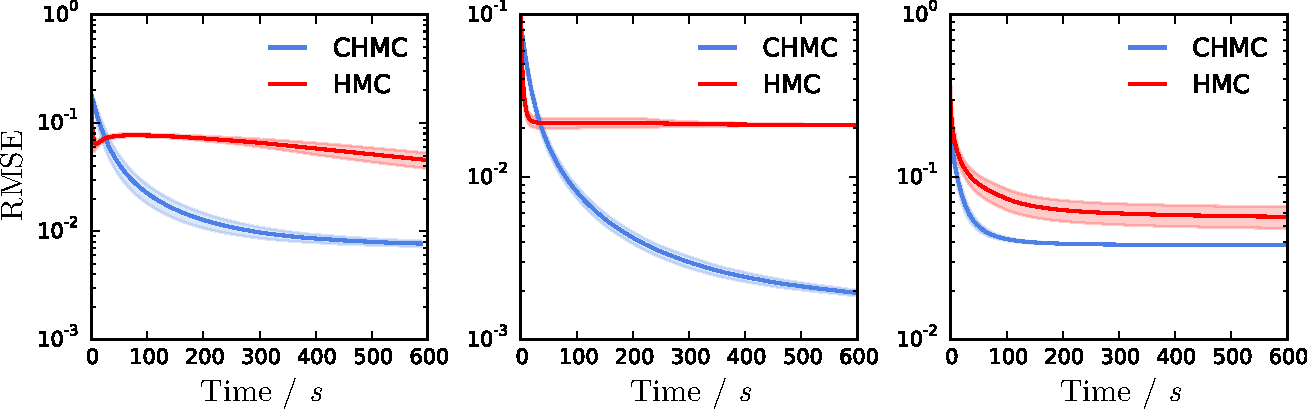
\includegraphics[width=\textwidth]{images/binocular-pose-estimates-rmse.pdf}
  \caption{}
  \label{sfig:pose-binocular-rmses}
\end{subfigure}
\\
\begin{subfigure}[b]{0.7\textwidth}
  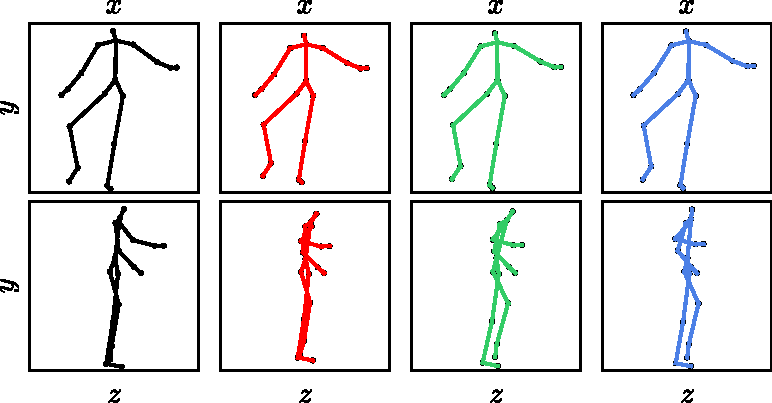
\includegraphics[width=\textwidth]{images/monocular-pose-sample-projections.pdf}
  \caption{}
  \label{sfig:pose-monocular-samples}
\end{subfigure}
\caption[Inference in human pose model.]{\textsf{Human pose}~ (a) \acp{RMSE} of 3D pose posterior mean estimates given binocular projections, using samples from our method (blue) versus running \ac{HMC} in hierarchical model (red) for three different scenes sampled from the prior. Horizontal axes show computation time to produce number of samples in estimate. Solid curves are average \ac{RMSE} over 10 runs with different seeds and shaded regions show $\pm 3$ standard errors of mean. (b) Orthographic projections (top: front view, bottom: side view) of 3D poses consistent with monocular projections. Left most pair (black) shows pose used to generate observations, right three show constrained \ac{HMC} samples.}
\label{fig:pose-inference}
\end{figure}

For our next experiment we considered inferring a three-dimensional human pose and camera model from two-dimensional projections of joint positions. We used a 19 joint skeleton model, with a learnt prior distribution over poses parametrised by 47 local joint angles $\rvct{z}_a$. The pose model was learnt from the \emph{PosePrior} motion capture data-set \citep{akhter2015pose} with a Gaussian \ac{VAE} \citep{kingma2013auto} trained to match the distribution of the motion capture joint angle data. The circular topology of the angular data is poorly matched by the Euclidean space a Gaussian \ac{VAE} typically learns a distribution on, and simply `unwrapping' the angles to e.g. $[-\pi,\pi)$ leads to unnatural discontinuities at the $\pm \pi$ cut-point, this both making the initial learning problem challenging (as there is no in-built prior knowledge of continuity across the cut-point) and tending to lead to a learned latent space less amenable to \ac{MCMC} inference as `nearby' poses with one or more joint angles on opposite sides of the cut-point will likely end up corresponding to points far apart in the latent space.

During training we therefore mapped each vector of 47 joint angles $\vct{z}_a^{(i)}$ (corresponding to a single motion capture datapoint) to a pair of 47-dimensional vectors $(\vct{r}_1^{(i)},\vct{r}_2^{(i)})$ by sampling a Gaussian random vector $\vct{n}^{(i)} \sim \nrm{\vct{0},\,\mathbf{I}}$ and then computing $\vct{r}_1^{(i)} = \exp\vct{n}^{(i)}\,\odot\,\cos\vct{z}_a^{(i)}$ and $ \vct{r}^{(i)}_2 = \exp\vct{n}^{(i)}\,\odot\,\sin\vct{z}^{(i)}_a$ and training the \ac{VAE} to maximise (a variational lower bound) on the joint marginal density of the $\lbrace \vct{r}^{(i)}_1,\,\vct{r}^{(i)}_2\rbrace_i$ pairs. At the cost of doubling the dimension, this leads to an embedding in a Euclidean space which does not introduce any arbitary cut-points and empirically seemed to lead to better sample quality from the learned generative model compared to learning the angles directly. Given the trained model we can generate a vector of angles $\rvct{z}_a$ using the model by sampling a Gaussian code (latent representation) vector $\rvct{u}_h$ from $\nrm{\vct{0},\mathbf{I}}$ then sampling a pair of 47-dimensional vectors $\rvct{r}_1$ and $\rvct{r}_2$ from the learnt Gaussian decoder model given $\rvct{u}_h$ (and further Gaussian random input vectors $\rvct{u}_1$ and $\rvct{u}_2$), and finally recovering an angle by computing $\rvct{z}_a = \textrm{atan2}(\rvct{r}_2,\rvct{r}_1)$. The resulting distribution on $\rvct{z}_a$ is only implicitly defined, but the overall generative model is differentiable with respect to the input vectors $\rvct{u}_h$, $\rvct{u}_1$ and $\rvct{u}_2$.

The \emph{PosePrior} motion capture data includes recordings from only a relatively small number of distinct actors and so limited variation in the `bone-lengths' of the skeleton model. Therefore a serparate log-normal model for the bone lengths $\rvct{z}_b$ was fitted using data from the \emph{ANSUR} anthropometric data-set \citep{gordon1988ansur}, due to symmetry in the skeleton thirteen independent lengths being specified. A simple pin-hole projective camera model with three position parameters $\rvct{z}_c$ and fixed focal-length was used\footnote{The camera orientation was assumed fixed to avoid replicating the degrees of freedom specified by the angular orientation of the root joint of the skeleton: only the relative camera--skeleton orientation is important.}. A log-normal prior distribution was placed on the depth co-ordinate $\rvar{z}_{c,2}$ to enforce positivity with normal priors on the other two co-ordinates $\rvar{z}_{c,0}$ and $\rvar{z}_{c,1}$. 

Given a generated triplet of joint-angles, bone length and camera parameters $\rvct{z}_a$, $\rvct{z}_b$ and $\rvct{z}_c$, a simulated two-dimensional projection of the skeleton $\rvct{x}$ is produced by first mapping the joint-angles and bone-lengths to a $4 \times 19$ matrix of joint positions $\rvct{P}$ in (homegeneous) world-coordinates by recursing through the skeleton tree. A $3 \times 4$ projective camera matrix $\rvct{C}$ is generated from $\rvct{z}_c$ and then used to project the world-coordinate joint positions to a $2 \times 19$ matrix $\rvct{X}$ of joint positions in two-dimensional image-coordinates. The projected positions matrix $\rvct{X}$ is flattened to a vector and a Gaussian vector with standard deviation $\epsilon$ added to the projected position vector to give the $19 \times 2 = 38$ dimensional observed vector $\rvct{x}$. The noise standard deviation $\epsilon$ is chosen so that the noise in the projected joint positions is non-obvious in generated projections. The overall corresponding model generator functions $\genfunc_{\rvct{x}|\rvct{z}}$ and $\genfunc_{\rvct{z}}$ are described procedurally in Algorithm \ref{alg:pose-model- generators} and a factor graph summarising the relationships between the variables in the model shown in Figure \ref{fig:pose-dgm-factor-graph}.

Although the Gaussian observed output noise is necessarily not needed to apply our proposed constrained \ac{HMC} method as the generator without the final additive noise still defines a valid differentiable generative model, using the noisy observation model means that an explicit hierarchical joint density on is defined on $\fset{\rvct{x},\,\rvct{u}_h,\,\rvct{r}_1,\,\rvct{r}_2,\,\rvct{z}_b,\,\rvct{z}_c}$ allowing comparison of our constrained \ac{HMC} method with (non-constrained) \ac{HMC} as a baseline. Further as discussed previously the adding noise to the output ensures the generator Jacobian is full-rank everywhere and also significantly simplifies the process of finding an initial $\rvct{u}$ such that the generated $\rvct{x}$ matches observations.

We first considered binocular pose estimation, with the variables defining the three-dimensional scene information $\rvct{z}_a$, $\rvct{z}_b$ and $\rvct{z}_c$, inferred given a pair of two-dimensional projections from two simulated cameras with a known offset in their positions (in this case the generator function is adjusted accordingly to output an $19 \times 2 \times 2 = 76$ dimensional observed vector $\rvct{x}$ corresponding to the concatenation of the flattened projected joint positions from both `cameras'). In this binocular case, the disparity in projected joint positions between the two projections gives information about the distances of the correspondings joints from the image plane in the depth direction and so we would expect the posterior distribution on the three-dimensional pose to be tightly distributed around the true values used to generate the observations. We compared our constrained \ac{HMC} method to running standard \ac{HMC} on the conditional density of $\fset{\rvct{u}_h,\,\rvct{r}_1,\,\rvct{r}_2,\,\rvct{z}_b,\,\rvct{z}_c}$ given $\rvct{x}$.

Figure \ref{sfig:pose-binocular-rmses} shows the \ac{RMSE} between the posterior mean estimate of the three-dimensional joint positions and the true positions used to generate the observations as the number of samples included in the estimate increases for three test scenes. For both methods the horizontal axis has been scaled by run time. The constrained \ac{HMC} method (blue curves) tends to give position estimates which converge more quickly to the true position. In this case standard \ac{HMC} performs relatively poorly despite the signficantly cheaper cost of each integrator step compared to the constrained dynamics. This is at leastin part due to the small output noise standard deviation $\epsilon$ used which requires a small integrator step to be used to maintain reasonable accept rates. Relaxing too larger $\epsilon$ values makes the non-constrained approach more competitive but with an associated cost in loss of 

 Visually inspecting the sampled poses and individual run traces (not shown) it seems that the \ac{HMC} runs tended to often get stuck in local modes corresponding to a subset of joints being `incorrectly' positioned while still broadly matching the (noisy) projections. The complex dependencies of the joint positions on the angle parameters mean the dynamic struggles to find an update which brings the `incorrect' joints closer to their true positions without moving other joints out of line. The constrained \ac{HMC} method seemed to be less susceptible to this issue.

We also considered inferring 3D scene information from a single 2D projection. Monocular projection is inherently information destroying with significant uncertainty to the true pose and camera parameters which generated the observations. Figure \ref{sfig:pose-monocular-samples} shows pairs of orthographic projections of 3D poses: the left most column is the pose used to generate the projection conditioned on and the right three columns are poses sampled using constrained \ac{HMC} consistent with the observations. The top row shows front $x$--$y$ views, corresponding to the camera view though with a orthographic rather than perspective projection, the bottom row shows side $z$--$y$ views with the $z$ axis the depth from the camera. The dynamic is able to move between a range of plausible poses consistent with the observations while reflecting the inherent depth ambiguity from the monocular projection.

\subsection{MNIST in-painting}

\begin{figure*}
\centering
\begin{subfigure}[b]{0.48\textwidth}
  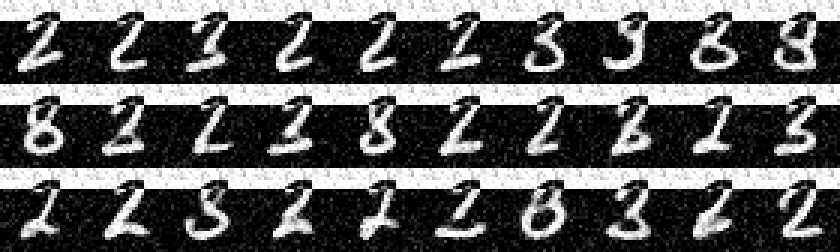
\includegraphics[width=\textwidth]{images/chmc-mnist-samples}
  \caption{Constrained HMC samples}
  \label{sfig:mnist-samples-chmc}
\end{subfigure}
~~
\begin{subfigure}[b]{0.48\textwidth}
  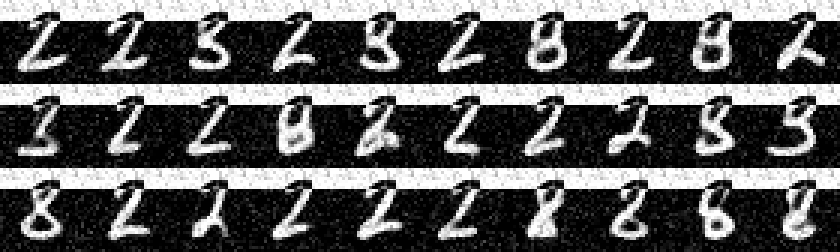
\includegraphics[width=\textwidth]{images/hmc-mnist-samples}
  \caption{HMC samples}
  \label{sfig:mnist-samples-hmc}
\end{subfigure}
\caption[MNIST in-painting samples.]{\textsf{MNIST}~ In-painting samples. The top black-on-white quarter of each image is the fixed observed region and the remaining white-on-black region the proposed in-painting. In left-right, top-bottom scan order the images in (a) are consecutive samples from a constrained \ac{HMC} run; in (b) the images are every 40\textsuperscript{th} sample from a \ac{HMC} run to account for the $\sim 40\times$ shorter run-time per sample. All images in this run are show in Figure \ref{fig:hmc-mnist-consecutive-states} in the Appendix.}
\label{fig:mnist}
\end{figure*}

As a final task we considered inferring in-paintings for a missing region of a digit image $\rvct{z}$ given knowledge of the rest of the pixel values $\rvct{x}$. A Gaussian \ac{VAE} trained on MNIST was used as the generative model, with a 50-dimensional hidden code $\rvct{h}$. We compared our method to running \ac{HMC} in the known conditional distribution on $\rvct{h}$ given $\rvct{x}$ ($\rvct{z}$ can then be directly sampled from its Gaussian conditional distribution given $\rvct{h}$).

Example samples are shown in Figure \ref{fig:mnist}. In this case the constrained and standard \ac{HMC} approaches appear to be performing similarly, with both able to find a range of plausible in-paintings given the observed pixels. Without cost adjustment the standard \ac{HMC} samples show greater correlation between subsequent updates, however for a fairer comparison the samples shown were thinned to account for the approximately $40\times$ larger run-time per constrained \ac{HMC} sample. Although the constrained dynamic does not improve efficiency here neither does it seem to hurt it.

\section{Discussion}

We have presented a generally applicable framework for performing inference in differentiable generative models. Though simulating the constrained Hamiltonian dynamic is computationally costly, the resulting coherent exploration of the state space can lead to significantly improved sampling efficiency over alternative methods.

Further our approach allows asymptotically exact inference in differentiable generative models where \ac{ABC} methods might otherwise be used. We suggest an approach for dealing with two of the key issues in \ac{ABC} methods --- enabling inference in continuous spaces as $\epsilon$ collapses to zero and allowing efficient inference when conditioning on high-dimensional observations without the need for dimensionality reduction with summary statistics (and the resulting task of choosing appropriate summary statistics). As well as being of practical importance itself, this approach should be useful in providing `ground truth' inferences in more complex models to assess the affect of the approximations used in \ac{ABC} methods on the quality of the inferences.

In molecular simulations, constrained dynamics are often used to improve efficiency. Intra-molecular motion is removed by fixing bond lengths. This allows a larger time-step to be used due to the removal of high-frequency bond oscillations \citep{leimkuhler2016efficient}. An analogous effect is present when performing inference in an \ac{ABC} setting with a $\epsilon$ kernel `soft-constraint' to enforce consistency between the inputs and observed outputs. As $\epsilon \to 0$ the scales over which the inputs density changes value in directions orthogonal to the constraint manifold and along directions tangential to the manifold increasingly differ. To stay within the soft constraint a very small step-size needs to be used. Using a constrained dynamic decouples the motion on the constraint manifold from the steps to project on to it, allowing more efficient larger steps to be used for moving on the manifold.

A limitation of our method is the requirement of differentiability of the generator. This prevents applying our approach to generative models which use discontinuous operations or discrete random inputs. In some cases conditioned on fixed values of discrete random inputs the generator may still be differentiable and so the proposed method can be used to update the continuous random inputs given values of the discrete inputs. This would need to be alternated with updates to the discrete inputs, which would require devising methods for updating the discrete inputs to the generator while constraining its output to exactly match observations.

As discussed in Section \ref{sec:abc}, a common approach in \ac{ABC} methods is to define the kernel or distance measure in terms of summary statistics of the observed data \citep{prangle2015summary,marin2012approximate}. This is necessary in standard \ac{ABC} approaches to cope with the `curse of dimensionality' with the probability of accepting samples / moves for a fixed tolerance $\epsilon$ exponentially decreasing as the dimensionality of the observations conditioned on increases. Although as already noted the proposed method is better able to cope with high observation dimensions, if appropriate informative statistics are available (e.g. based on expert knowledge) and these are differentiable functions of the generator outputs, they can be easily integrated in to the proposed method by absorbing the statistic computation in to the definition of $\genfunc_{\rvct{x}}$.
